\documentclass[a4paper, 12pt]{article}

%%%%%%%%%%%%
% Packages %
%%%%%%%%%%%%

\usepackage[english]{babel}
\usepackage{packages/sleek}
\usepackage{packages/sleek-title}
\usepackage{float}
\usepackage{listings}
\usepackage{xcolor}

\colorlet{mygray}{black!30}
\colorlet{mygreen}{green!60!blue}
\colorlet{mymauve}{red!60!blue}

\lstset{
  backgroundcolor=\color{gray!10},  
  basicstyle=\ttfamily,
  columns=fullflexible,
  breakatwhitespace=false,      
  breaklines=true,                
  captionpos=b,                    
  commentstyle=\color{mygreen}, 
  extendedchars=true,              
  frame=single,                   
  keepspaces=true,             
  keywordstyle=\color{blue},      
  language=c++,                 
  numbers=none,                
  numbersep=5pt,                   
  numberstyle=\tiny\color{blue}, 
  rulecolor=\color{mygray},        
  showspaces=false,               
  showtabs=false,                 
  stepnumber=5,                  
  stringstyle=\color{mymauve},    
  tabsize=3,                      
  title=\lstname                
}



%%%%%%%%%%%%%%
% Title-page %
%%%%%%%%%%%%%%

\logo{./resources/logo.png}
\institute{Cambridge University}
\faculty{Part II Physics: Computing Project}

\title{The Ising Model of a Ferromagnet}

\author{\textit{BGN:}\ \textsc{7005W}}
\date{\today}


%%%%%%%%%%%%
% Document %
%%%%%%%%%%%%

\begin{document}
    \maketitle
    
        \begin{abstract}
    This report delves into using a computational approach to simulating a ferromagnet using the Ising model and measuring its characteristics with statistical analysis. The program, implemented in C++ can simulate the evolution of a spin lattice and calculate macroscopic properties such as magnetisation, susceptibility, heat capacity and others. The critical phase transition temperature was measured up to a lattice of size \(N = 400\) with a value \(T_c(N=400) = 2.2690 \pm 0.0015 \) which is in agreement with analytically derived values for the Ising model. The computational efficiency of the program was investigated and optimised to allow simulations of larger lattices to higher accuracy. A single core of an AMD Ryzen 5 CPU was used for running computations and for a lattice of size \(N=400 \) the number of steps required to achieve convergence of results was 200,000, totalling over 3 hours of run time per temperature. 
    \end{abstract}
    
    \romantableofcontents
    
    \section{Introduction}
    \subsection{Ising Model}
	The Ising Model is a simple statistical model which aims to represent a ferromagnetic material. The model considers a 2 dimensional lattice of spins pointing either up or down with simple dynamics governing how the spins evolve.	
\begin{figure}[H]
\centering
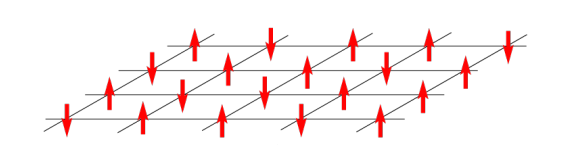
\includegraphics[width=0.75\textwidth]{./resources/ising_model.png}
\caption{Ising Model Lattice}
\end{figure}
The remarkably simple model predicts many features of real ferromagnetic materials including first and second order phase transitions, thermodynamic properties, and hysteresis effects. These phenomena will be investigated and quantified using the Ising Model, as well as their error compared to analytical models.

	\subsection{Metropolis Algorithm}
The Metropolis algorithm is a Monte Carlo approach that dictates how the dynamics of the spin lattice evolves. The following convention for terms will be used throughout.

For a 2 dimension lattice of linear size \(N\), there are \(N^2\) total spins \(s_i\). The energy of the system is defined as
\[ E = - J  \sum_{(ij)}{s_i s_j} - \mu H \sum_{i=1}^{N^2} s_i \]
where \( (ij) \) is the sum over nearest neighbour pairs of spins, four total in the 2D case. The external magnetic field applied is \( H \) and the constants \(J\) and \( \mu \) represent physical parameters of the system. 

To simplify analysis, the constants are incorporated into the units of the other dynamical variables. Magnetic field is measured in units \(1 / \mu \) and temperature is measured in units of constants \( J / k_B \). Therefore these parameters may be set to unity \(J = \mu = 1\). 

For reference, in reduced units Onsager's analytical result for critical temperature is \( T_c = 2/\ln(1+\sqrt(2)) \approx 2.26918 \) \cite{1}.

The metropolis algorithm for lattice evolution is as follows
\begin{enumerate}
  \item Select a spin. Calculate \( \Delta E \) to flip it.
  \item If \( \Delta E < 0 \) flip the spin.
  \item If \( \Delta E > 0 \), select a random number \(p \in [0,1] \).
  \item If \( \exp(- \Delta E / (k_B T) ) > p \), flip the spin.
\end{enumerate}

This process is repeated for \(N^2\) spins, after which constitutes a single {\it Monte Carlo time step} (time-step or time). There are two approaches for selecting spins, either iteratively going through the lattice or picking a spin at random. The performance characteristics of the metropolis algorithm and different spin selection methods will be further investigated.


    \newpage
    \section{Computational Analysis}
    

	\subsection{Memory Scaling}
	The main memory constraints are storing the state of each lattice spin and keeping a record of the magnetisation at each time-step throughout the simulation. For a lattice of size \(N\) running for \(t\) steps, the memory usage to therefore scales as \(O(N^2 + t)\). In the case of a very large lattice \(N=1000\) running for \(t=10,000\) steps, with each spin represented by one byte and magnetisation stored with eight bytes, the total memory usage is approximately \(1MB\) which is very much within modern computing capability. Therefore the memory constrains can be ignored and only the time constraints need be considered.

	\subsection{Time Scaling}
	At each time step, the simulation must perform a spin flip check for each of the \(O(N^2)\) lattice sites. Therefore the total time complexity is \(O(t N^2)\) which grows much faster than the memory usage. Combined with critical slowing down of the metropolis algorithm near transition points, the time scaling of the problem is the most significant constraint. This motivates a very fast implementation of the metropolis algorithm, which will allow for larger lattices to be investigated with higher accuracy. Additionally, the metropolis algorithm cannot be vectorised as it requires accessing of its neighbours' state. 

	\subsection{C++ vs Python}
	The decision to use C++ or Python to implement the model involves a few considerations. As C++ is a low level language, it has very fast execution of basic routines such as loops and arithmetic operations, compared to Python's which can be over 100x slower \cite{2}. However this comes with a trade off of more complexity and effort to implement algorithms. The main numerical routine of the metropolis is a set of nested loops, making C++ the clear choice to maximise the speed of execution. 

	\newpage
	\subsection{Initial Lattice State}
	The initial lattice state can either be all spins randomly oriented, or all pointing in the same direction. To test which option is more suitable, the time taken to converge to equilibrium is investigated. The comparison of a uniform lattice \(M(0)=1\) to a random initial lattice \(M(0) \approx 0 \) is shown below. 

\begin{figure}[H]
\centering
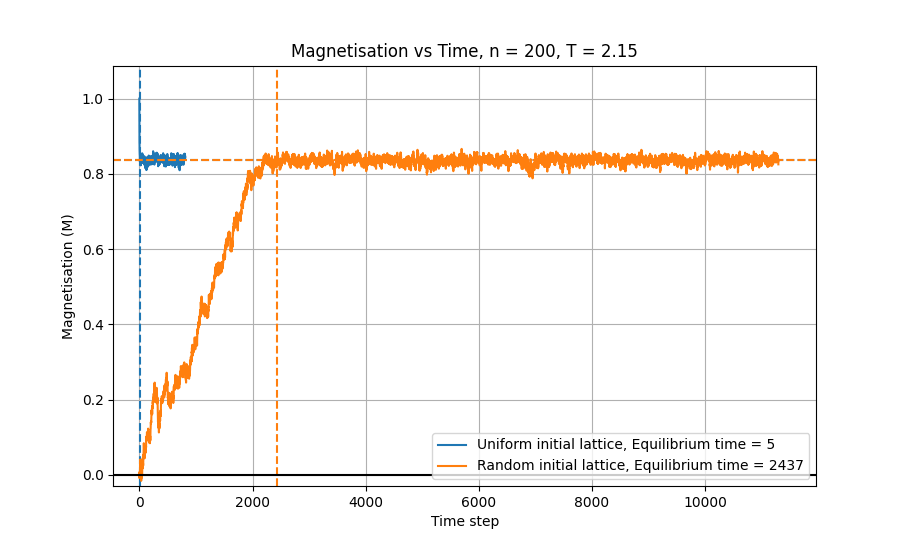
\includegraphics[width=0.75\textwidth]{./resources/random_vs_uniform.png}
\caption{Random initial lattice vs Uniform initial lattice}
\end{figure}

From the above plot, it is clear the uniform lattice converges to equilibrium significantly faster (indicated by vertical lines). Furthermore, after convergence both lattices have the same mean magnetisation, confirming that the initial state does not affect the final results. Therefore, a uniform lattice is chosen as the initial state for all simulations to maximise speed. 

	\subsection{Correlation Time}
The auto-covariance of magnetisation is defined by
\[ A( \tau ) = \left< M'(t) M'(t + \tau) \right> \]
where
\[ M'(t) = M(t) - \left< M(t) \right> \]
The autocorrelation is then given by
\[ a(\tau) = \frac{A(\tau)}{A(0)} \]

The time taken for the autocorrelation to fall to \( \tau_e = 1/e\) is the decorrelation time, quantifying how long the system takes for the parameter to propagate throughout the lattice. It is important to measure the decorrelation time, as before this time the system is still settling and any statistical measurements will have a systematic error. The autocorrelation with their decorrelation times are plotted for a range of temperatures.

\begin{figure}[H]
\centering
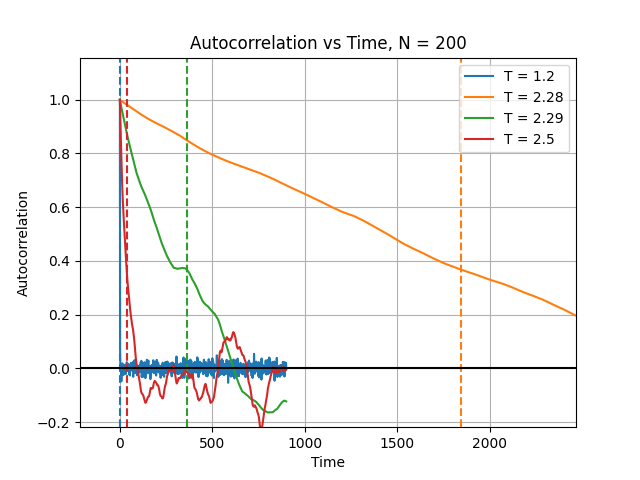
\includegraphics[width=0.75\textwidth]{./resources/decorrelation_time.png}
\caption{Autocorrelation vs Time for lattice \(N=100\) for a range of temperatures}
\end{figure}

At temperatures above and below critical points, the decorrelation time is very short. However near the transition point the decorrelation time grows very large. To ensure statistical results have settled, all simulations are run for minimum of ten times the decorrelation time \(t_{total} = 10\tau_e \).

	\subsection{Critical Slowdown}
The metropolis algorithm suffers from rapidly increasing correlation times near criticality, with the increase of lattice size. To quantify this effect, the decorrelation time at critical temperature is measured for a range of lattice sizes and shown on a log-log plot.

\begin{figure}[H]
\centering
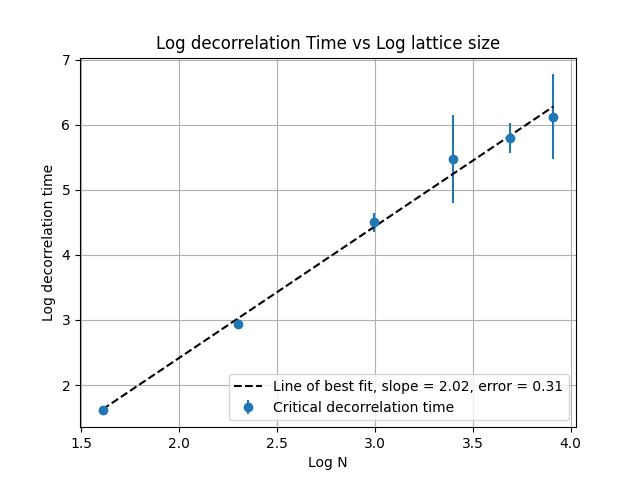
\includegraphics[width=0.75\textwidth]{./resources/critical_slowdown.png}
\caption{Critical Slowdown. Log-log plot of decorrelation time at critical temperature versus lattice size}
\end{figure}

The dynamic exponent \(z\) determines the scaling relation for decorrelation time \(\tau_e \sim N^z \) where \( z = 2.02 \pm 0.31 \) is the measured value. This is within the agreed value for the metropolis algorithm \(z_{met} = 2.166 \) according to literature \cite{3}.

Furthermore, with this result it is clear that the required simulation steps to have correlated results also scales with lattice size. Combined with the previous effect, this can put a lower bound on the total time complexity.
\[ t \sim O(N^{2+z}) = O(N^{2.02}) \]
This concludes that the simulation time grows at least to the fourth power with lattice size.

    \newpage
    \section{Implementation}

	\subsection{Code Structure}
	The structure of the main C++ source code is illustrated in the UML diagram below.
\begin{figure}[H]
\centering
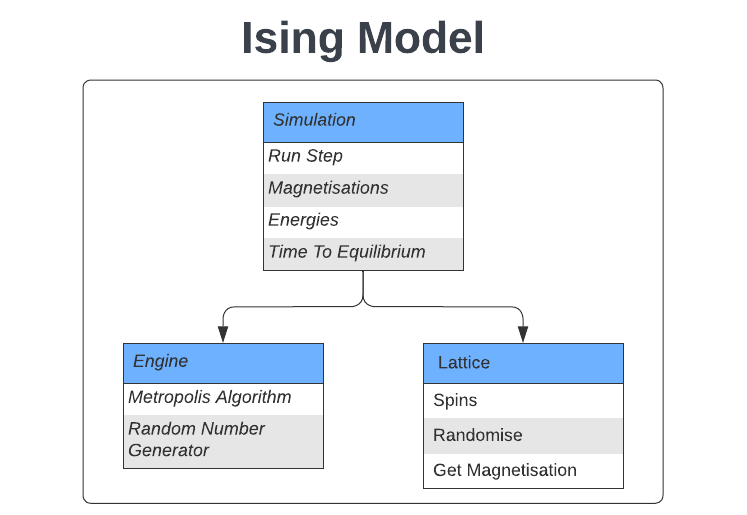
\includegraphics[width=0.75\textwidth]{./resources/ising_UML_diagram.png}
\caption{Ising Model UML diagram}
\end{figure}
	
	\subsubsection{Ising Model Source}
	The Ising Model is implemented in three classes, with the main point of access being {\it Simulation}. 
	\begin{itemize}
		\item {\it Lattice} is simply a wrapper for the matrix of spins. It provides helper functions for commonly used routines such a randomise, get magnetisation, and get energy. 

		\item {\it Engine} contains the implementation of the metropolis algorithm and is mainly used to get the next time step of the lattice, while hiding the implementation details. It contains optimised routines for generating random numbers and calculating spin flipping.

		\item {\it Simulation} keeps track of the history of the simulation. It is used to set the size, temperature, and external field of the lattice. At each time step, it records lattice properties such as magnetisation and energy.
	\end{itemize}

\begin{figure}[H]
\centering
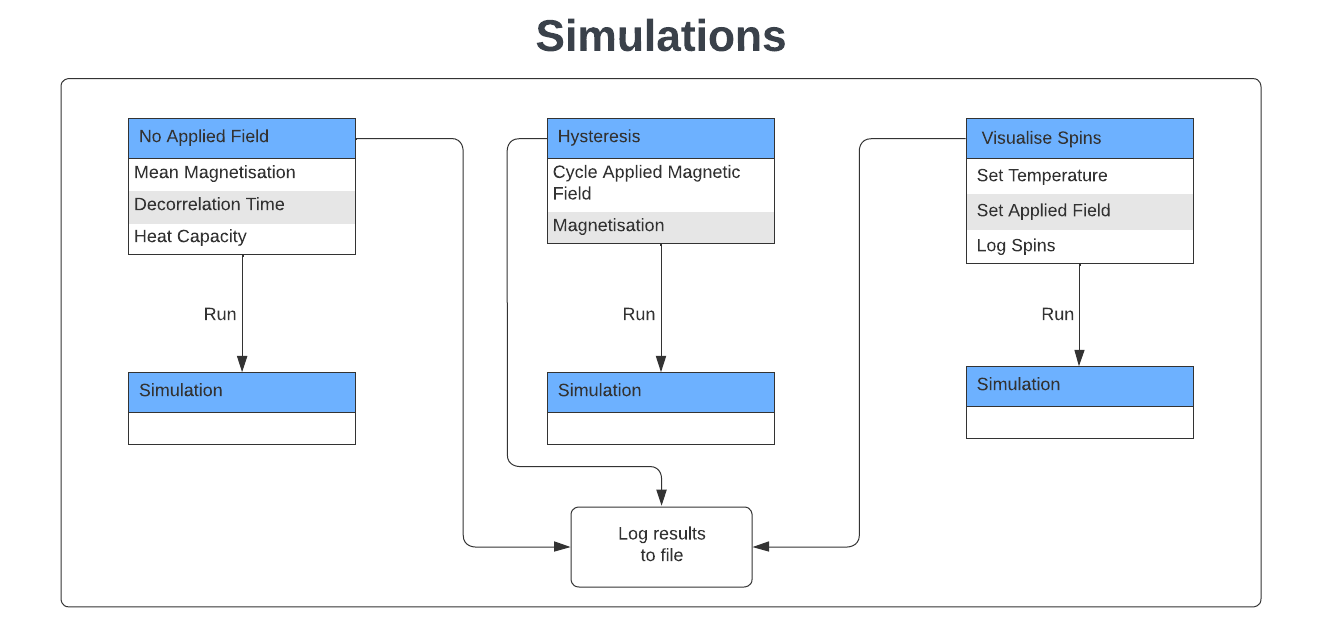
\includegraphics[width=\textwidth]{./resources/sim_UML_diagram.png}
\caption{Simulations UML diagram}
\end{figure}
	

	\subsubsection{Simulations Source}
	The simulations implement the specific details of each experiment that is to be run and then logs the results to a file for later analysis. 
	\begin{itemize}
		\item {\it No Applied Field} is the basic simulation with no external field. For varying lattice sizes and temperatures, it calculates statistical properties including mean magnetisation, decorrelation time, heat capacity, and critical temperature.

		\item {\it Hysteresis} implements a simulation where an external magnetic field is cycled over the lattice and the resulting magnetisations are measured. 

		\item {\it Visualise Spins} is a simulation which logs the spins of the entire lattice under different situations such as cooling and cycling of external field. The spins are then used to reconstruct an image of the lattice in these regimes.
	\end{itemize}

	\subsubsection{Scripts}
	There is also a scripts folder, where each simulation has an accompanying Python script that reads and sorts the data produced by the simulation. Then the results are plotted in an appropriate graph. All figures in this report were created by these scripts.

	\newpage
	\subsection{Calculating Time To Equilibrium}
	It is important to calculate when the lattice has reached equilibrium, as the properties of the model can only be measured after this point. The algorithm for calculating time to equilibrium aims to measure when the energy of the system has stabilised. 

A sliding window calculates the line of best fit for energy in the interval \([t_i, t_i + \text{offset}]\). Once the gradient of the line of best fit is below some threshold value, equilibrium is reached. The idea is that once energy has stabilised, the line of best fit will be flat. 

This approach benefits from not being sensitive to the size of fluctuations in energy, as the line of best fit will be balanced to zero. The size of the window used is a tenth of the total time, which provides very accurate estimates of the time to equilibrium as shown below.
\begin{figure}[H]
\centering
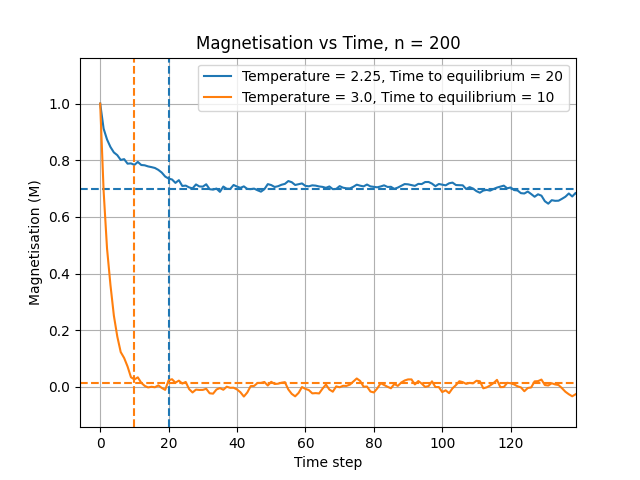
\includegraphics[width=0.75\textwidth]{./resources/magvstime_2T.png}
\caption{Magnetisation vs Time showing convergence to equilibrium. Vertical lines show when equilibrium is detected. Horizontal lines show mean magnetisation after equilibrium.}
\end{figure}




    \newpage
    \section{Performance}
\subsection{CPU Time}
Computational performance was tested by measuring the total computation time of running 10,000 steps for a range of lattice sizes. A single core on an AMD Ryzen 5 CPU was used for running simulations.

The iterative algorithm of stepping through the lattice to select spins to flip is compared to a Monte Carlo approach of randomly selecting spins. A log-log plot of total computation time versus lattice size is shown below.
\begin{figure}[H]
\centering
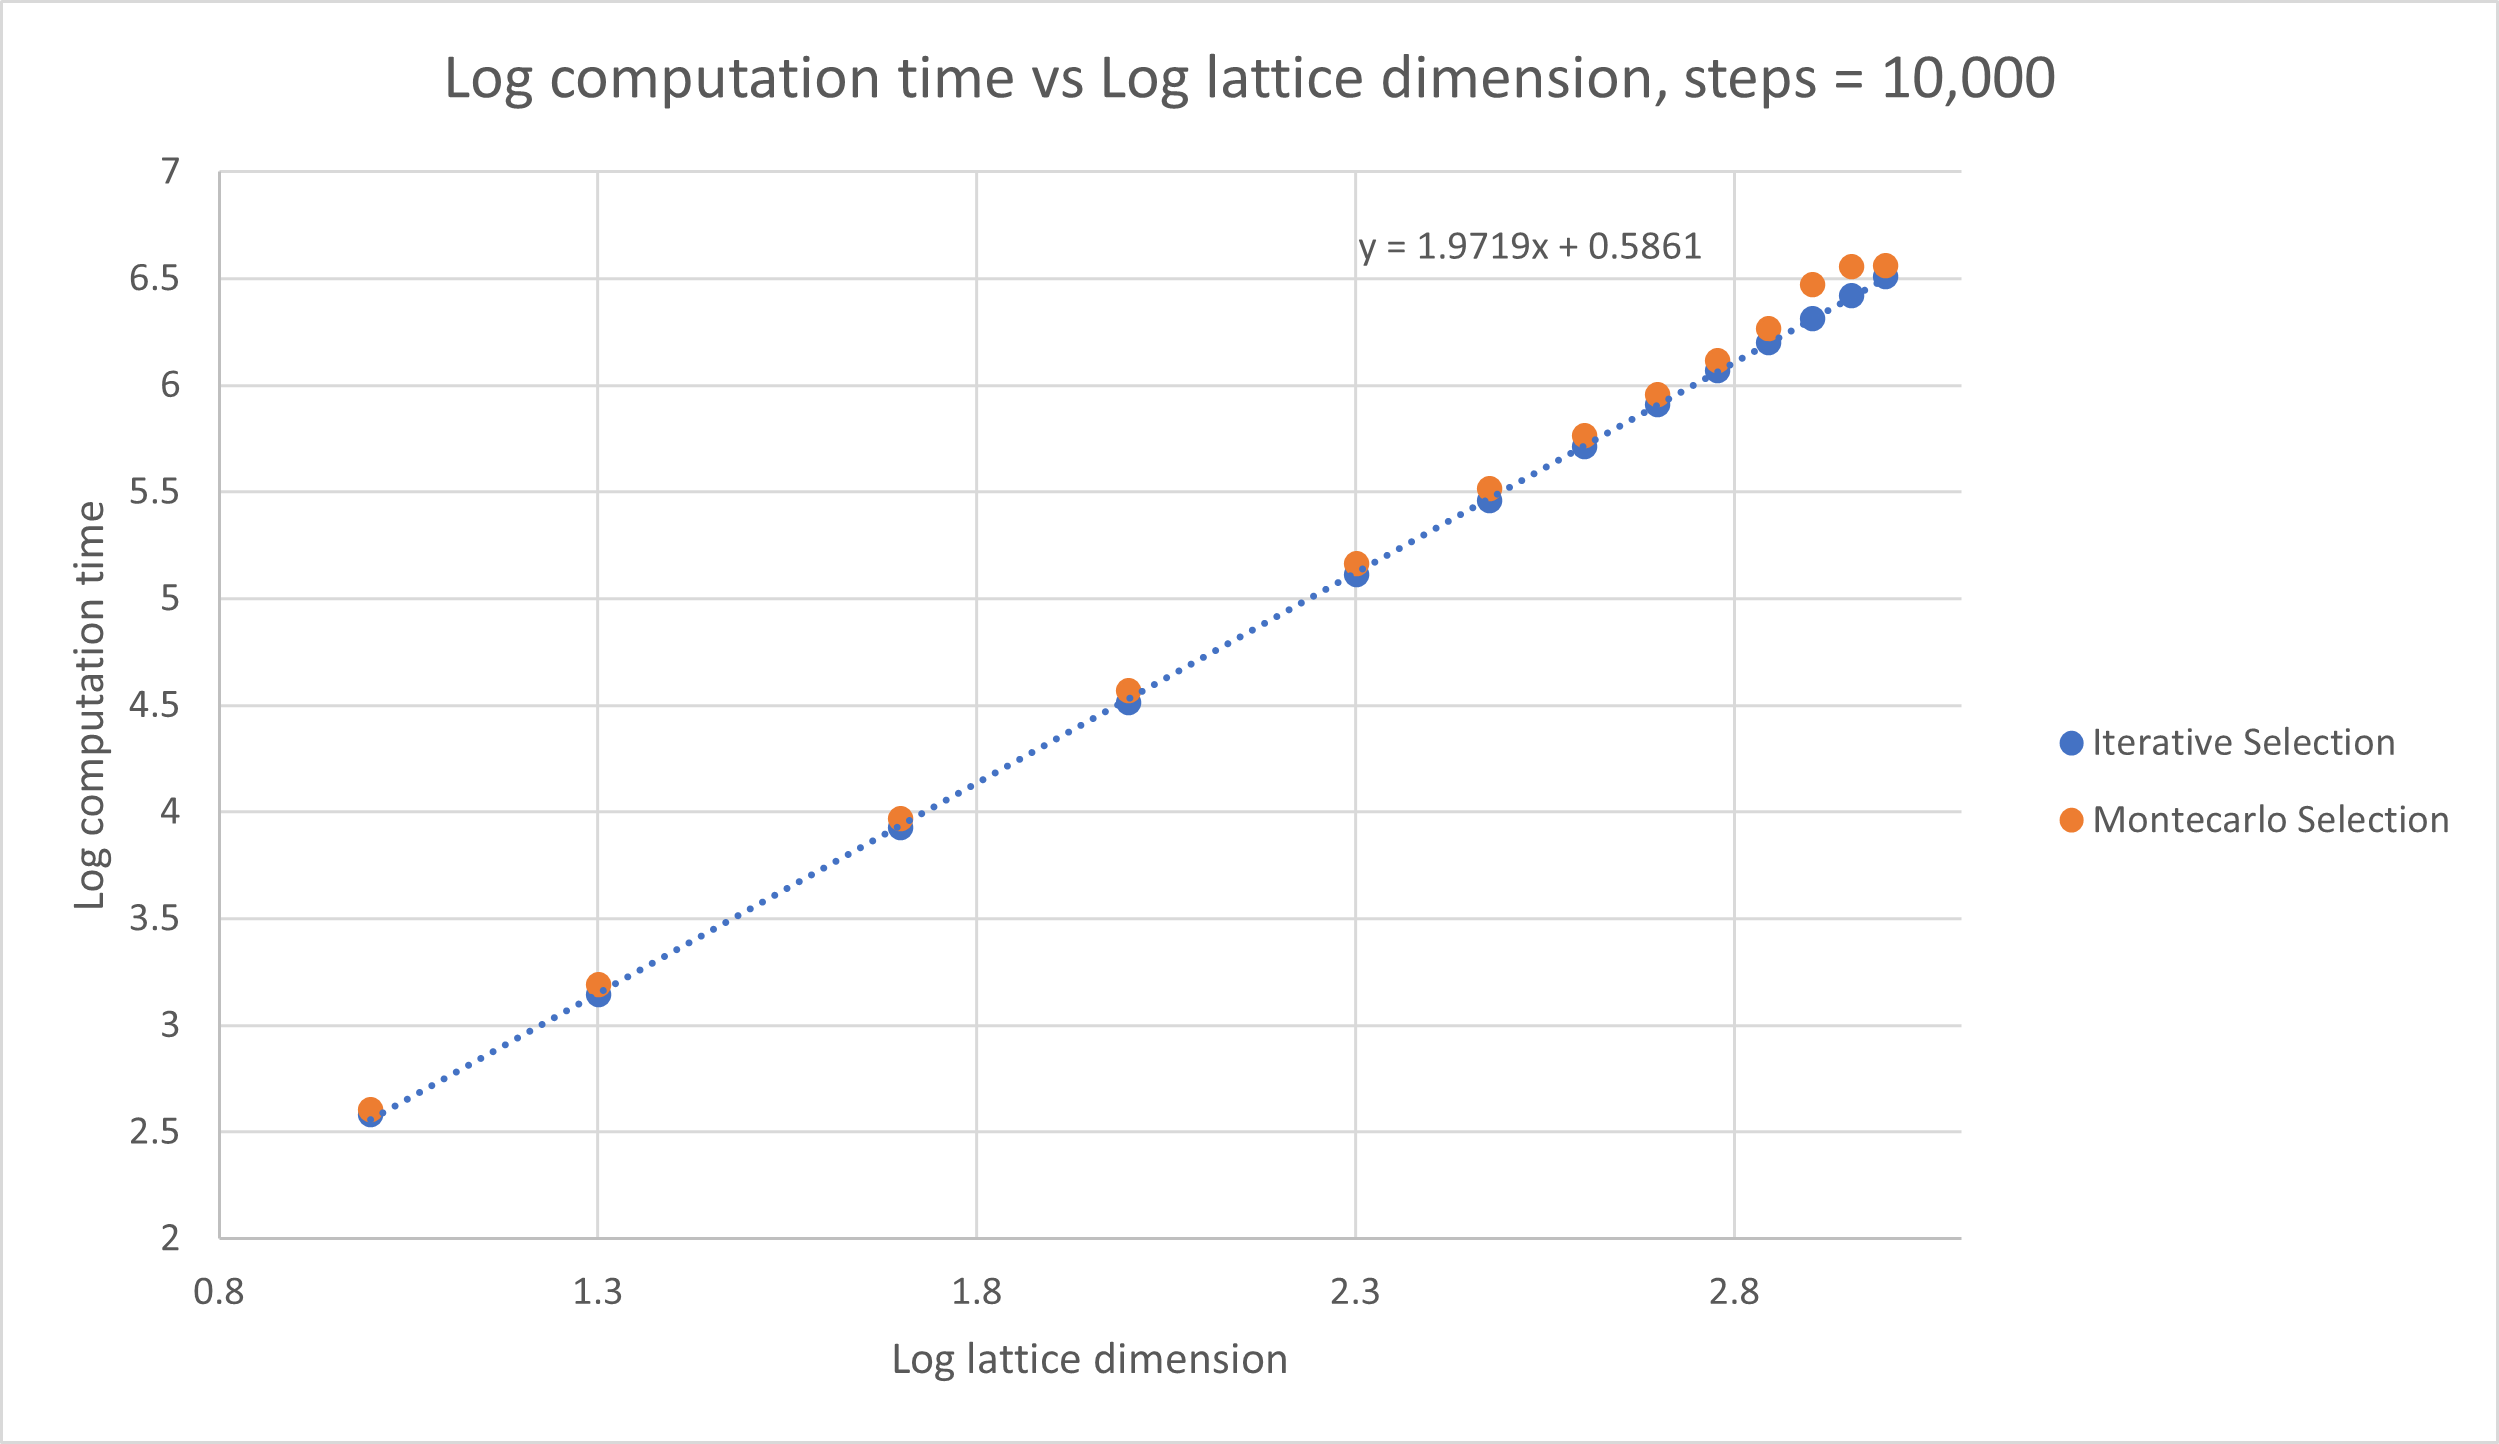
\includegraphics[width=0.75\textwidth]{./resources/log_computation_time.png}
\caption{Log-log plot for computation time versus linear lattice dimension}
\end{figure}

The iterative approach is slightly faster as no time is spent generating additional random numbers, however the difference is small. As expected, the gradient is approximately 2, verifying the computational complexity is \( O(N^2) \). The raw time in minutes is shown below for each lattice. 

\begin{figure}[H]
\centering
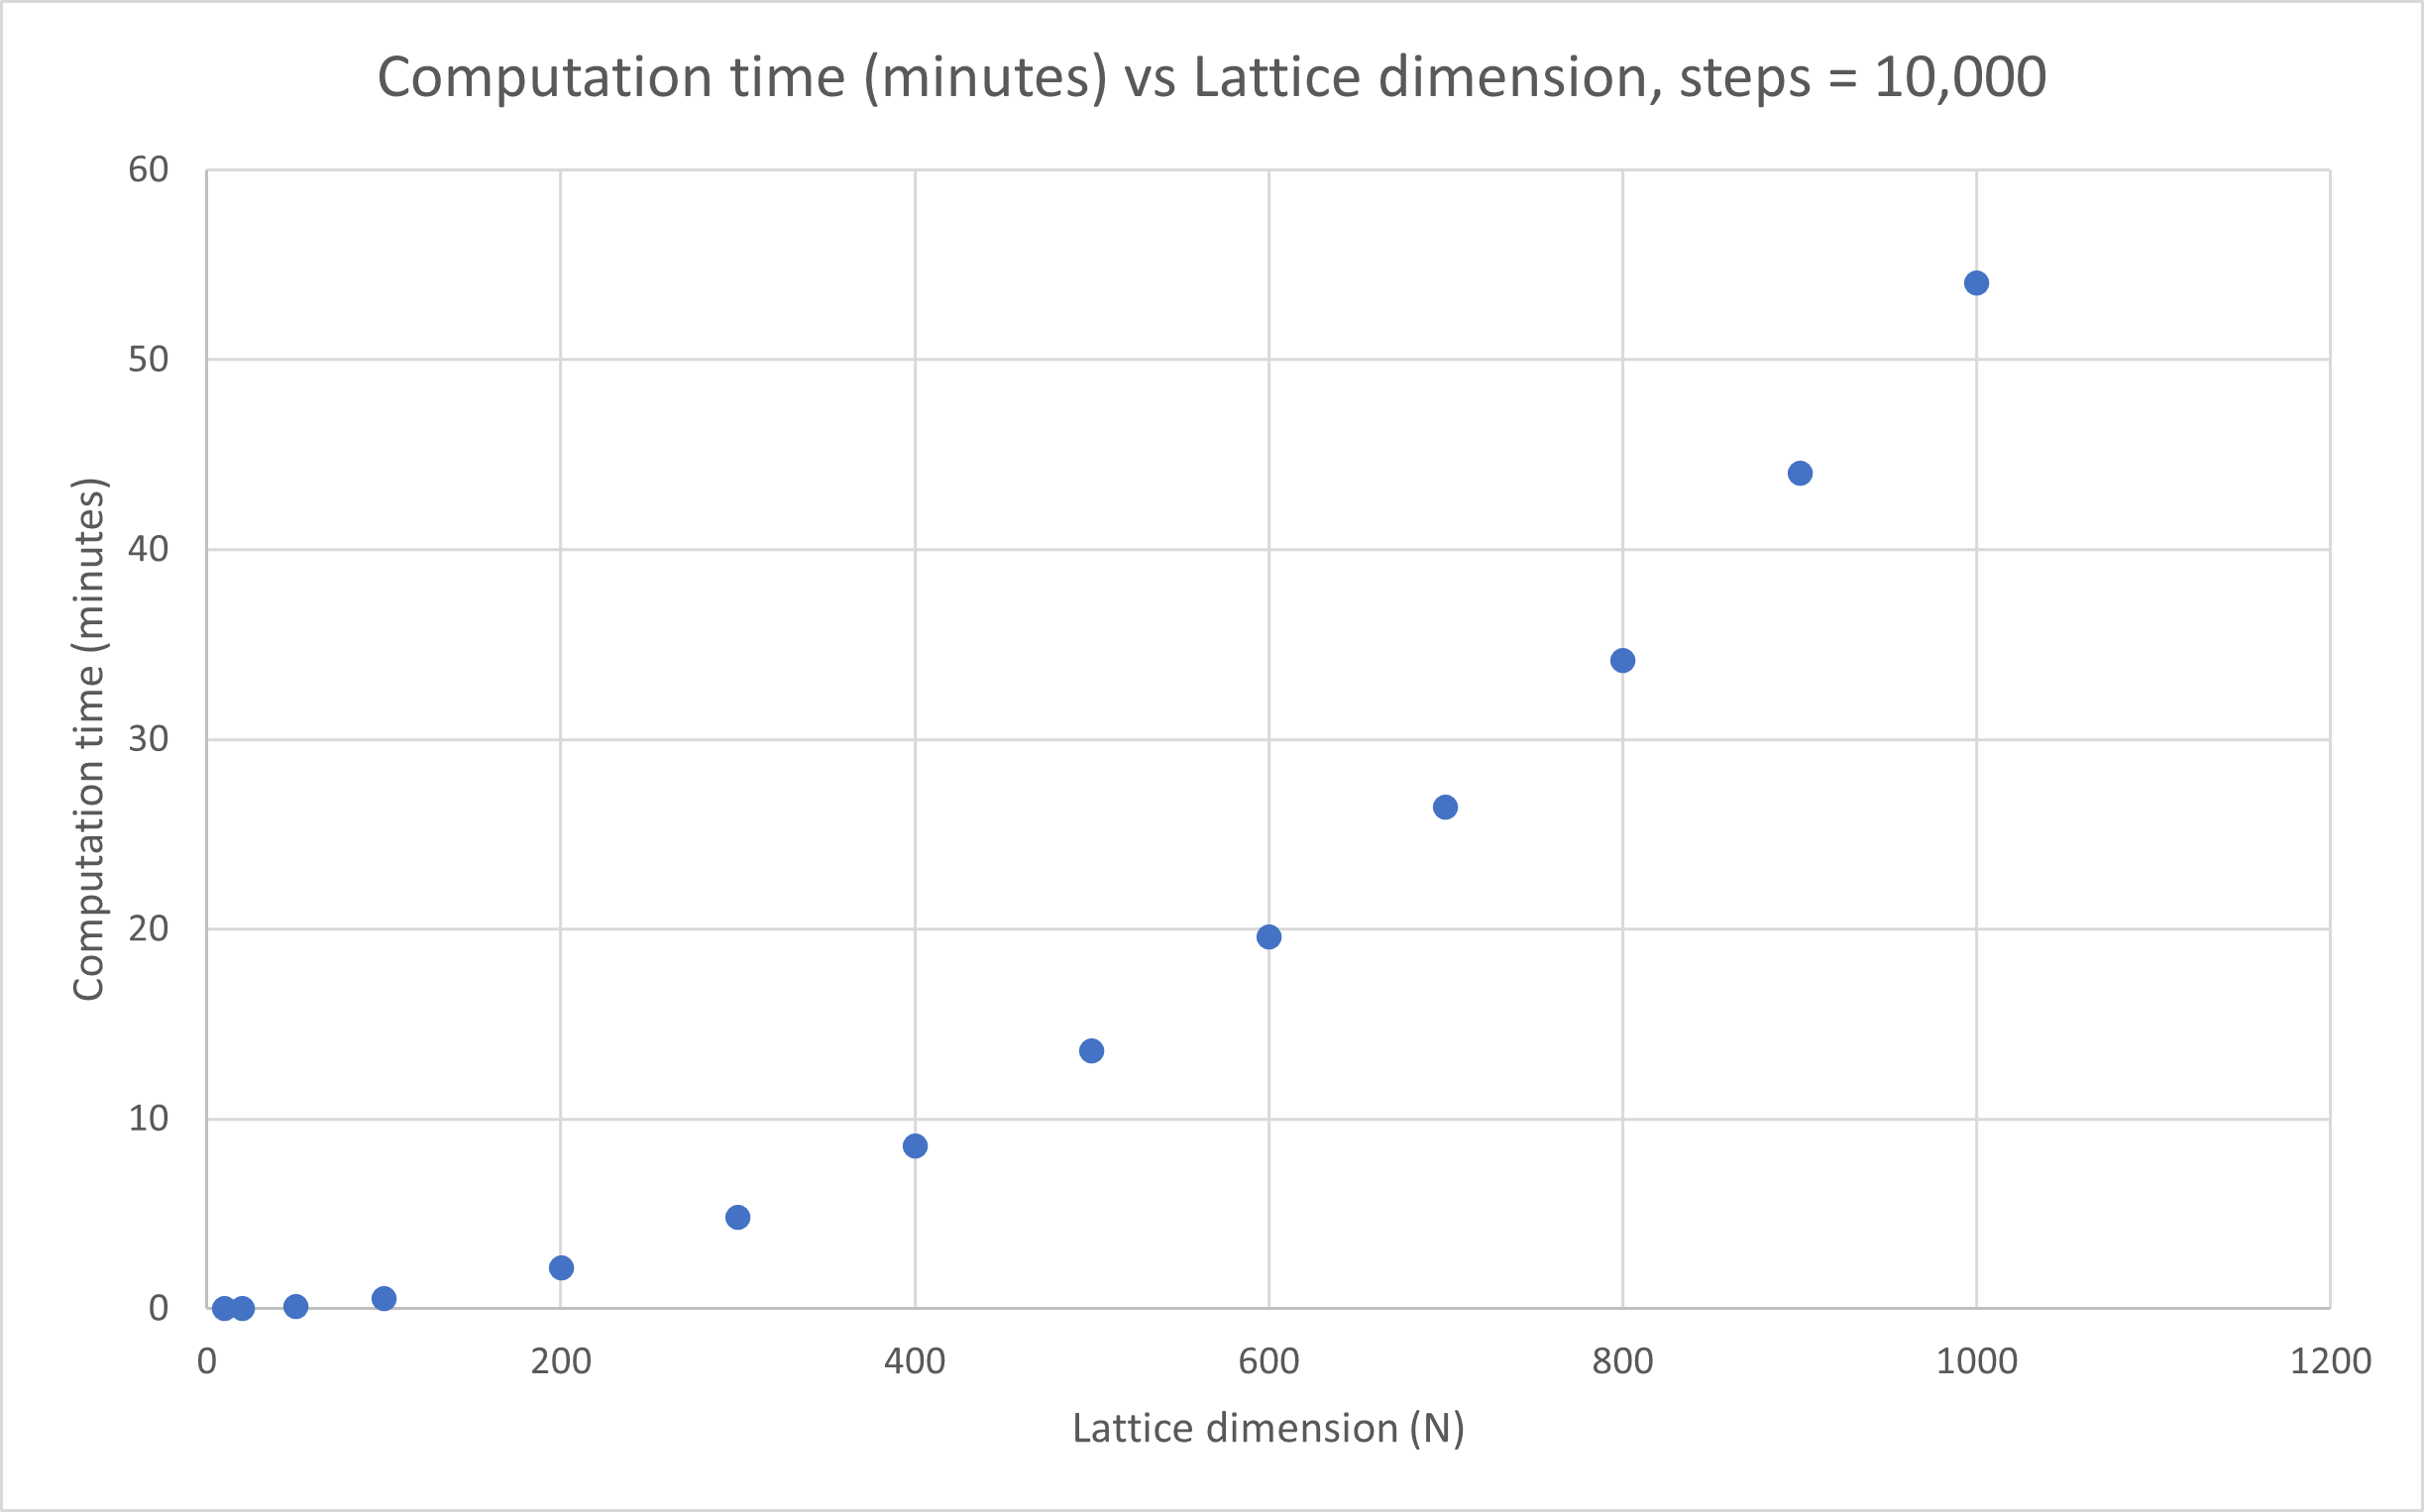
\includegraphics[width=0.75\textwidth]{./resources/raw_computation_time.png}
\caption{Time in minutes taken to simulate 10,000 steps for range of lattice sizes}
\end{figure}

For the largest lattice, \(N=1000\) the total time taken was approximately an hour, which gives an average speed of 360 milliseconds per step. 

To collect results, each lattice was swept over a range of fifty temperatures for a minimum of 5,000 steps. Each simulation is then repeated ten times to gather a sample giving a more accurate mean and an estimation of the error. The largest lattice used in this process was for \( N= 200 \), and it takes over 8 hours in total.

For measuring critical temperature, the largest lattice size of \( N = 400 \) required simulations of up to 200,000 steps to achieve convergence. As this process can take over 3 hours per temperature, only a few temperatures near the critical point were calculated.  

Code performance was optimised by carefully implementing functions to be as efficient as possible. This includes avoiding making unnecessary copies, not repeating work, and using fast random number generators. There is no single optimisation, but rather a collection of well tested, fast C++ code.


\subsection{Dynamic runtime}
There is large variation in the time to convergence between all the simulations, with critical slowing down at the transition points. Rather than manually selecting the total number of steps to run each simulation, an algorithm dynamically increases total simulation time. This is achieved by ensuring the total simulation steps is at least ten times the decorrelation time, \( t_{total} = 10 \tau_e \). This feature can be seen in the range of total simulation time below, with vertical lines showing when equilibrium is detected. 
\begin{figure}[H]
\centering
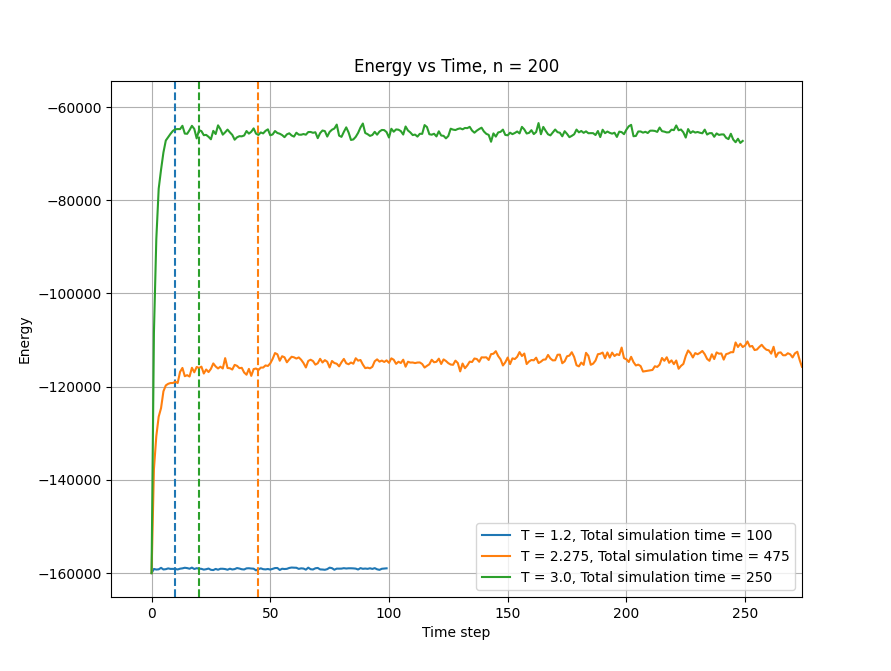
\includegraphics[width=0.75\textwidth]{./resources/energy_vs_time.png}
\caption{Energy vs Time with dynamic simulation time}
\end{figure}

This approach means that near critical points, the program automatically runs for longer time to ensure all interesting features are measured. Furthermore, it avoids wasting unnecessary computation time once a simulation has converged, increasing performance on a large set of calculations. 



\newpage
\section{Results and Discussion}

\subsection{Mean magnetisation}
One of the primary features of the Ising model is the prediction of phase transitions in order parameters. The magnetisation, calculated as the mean spin of the model, displays this transition as a function temperature. The mean absolute magnetisation versus temperature and associated errors with no external field applied is shown below.

\begin{figure}[H]
\centering
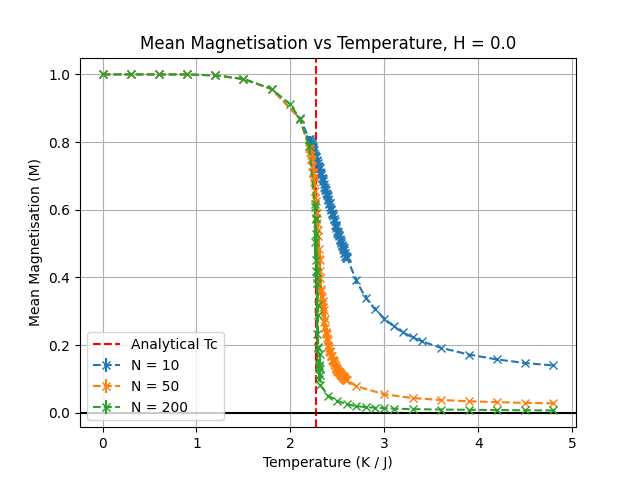
\includegraphics[width=0.75\textwidth]{./resources/mag_vs_temp.png}
\caption{Magnetisation versus Temperature for three lattice sizes, with analytical critical temperature indicated}
\end{figure}

The magnetisation displays characteristics expected of a second order phase transition, with the magnetisation continuously going to zero above the critical temperature. It is also evident that the transition becomes more discrete as the lattice size increases.

Near the critical temperature, symmetry breaking is observed over the course of a simulation. Starting from a spin up magnetised lattice, the magnetisation has a small probability to randomly break symmetry and align to spin down. The plot below shows the evolution of magnetisation for temperature \( T = 2.25 < T_c \).

\begin{figure}[H]
\centering
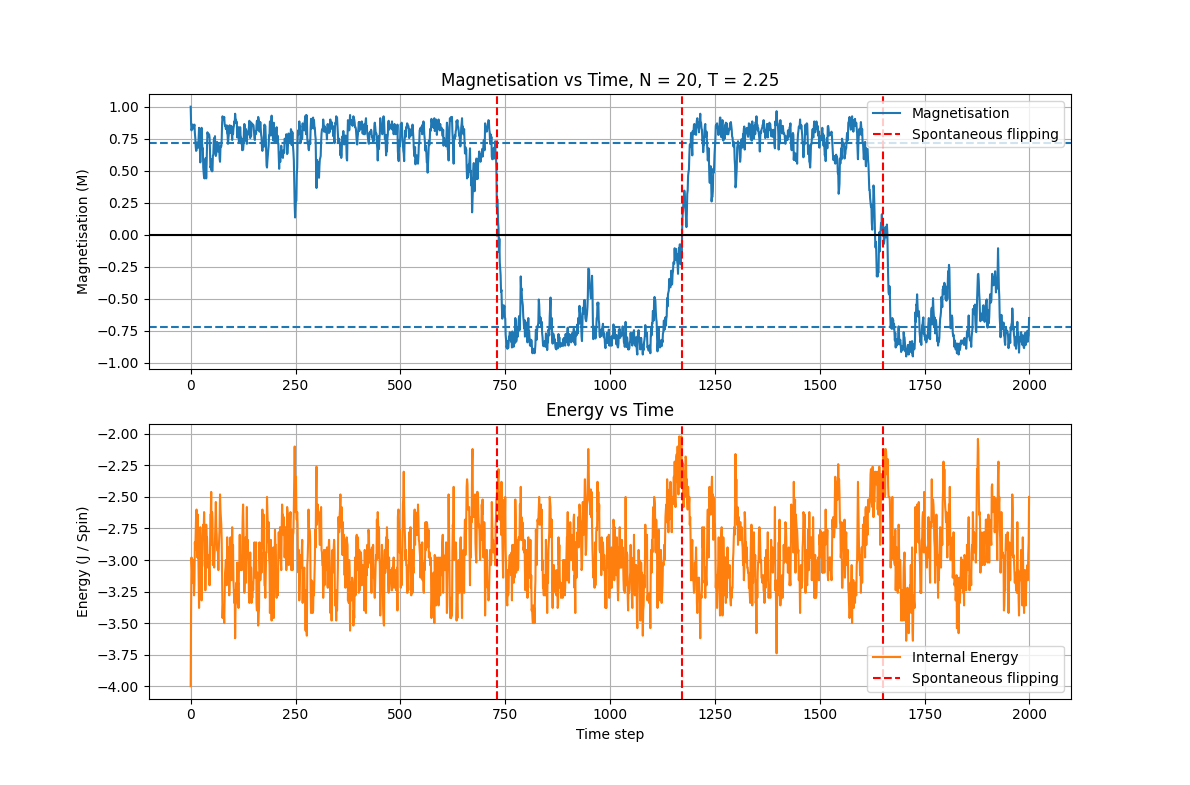
\includegraphics[width=\textwidth]{./resources/symmetry_breaking.png}
\caption{Magnetisation symmetry breaking near critical temperature and associated internal energy.}
\end{figure}

The magnetisation spontaneously changes three times, with each flipping having an associated spike in internal energy. This effect becomes less probable as the lattice size increases, as a larger bump in energy is required to have a spontaneous flipping. This is also a result of critical slowing and longer simulation times become required for symmetry breaking to occur with increasing lattice size. 


\subsection{Heat Capacity}
The fluctuation dissipation theorem states that the variance in system energy is related to the heat capacity of the system \cite{4}. The exact relation is given by 
\[C = \frac{\sigma_E^2}{(k_B T)^2} \]
Where \( \sigma_E^2 \) is the internal energy variance, \( T \) is the temperature, and \( k_B = 1 \).

The measured heat capacity per spin and calculated errors are plotted below for a range of lattice sizes. The analytical solution for heat capacity of the 2D Ising model is given by \cite{5} and is included in the plot
\[C \propto -\log(|T-T_c|) \]

\begin{figure}[H]
\centering
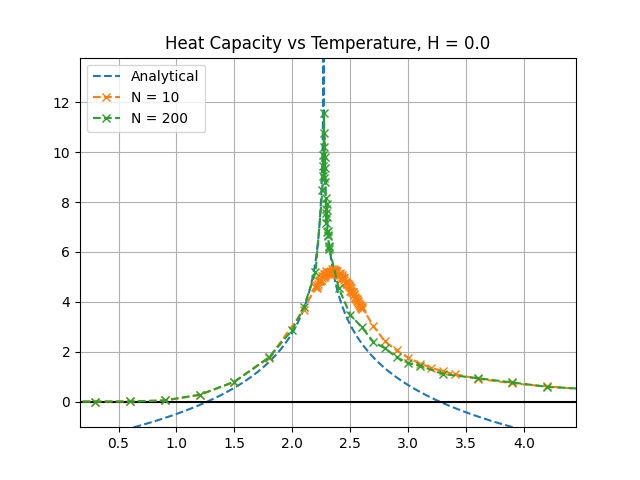
\includegraphics[width=0.75\textwidth]{./resources/heat_capacity.png}
\caption{Measured heat capacity versus temperature for two different lattice sizes. Included is the analytical solution}
\end{figure}

As the lattice size increases, the heat capacity curves become more similar to the analytical solution, with sharper peaks corresponding to the critical temperature. Each temperature is simulated ten separate times and the error in the heat capacity is calculated as the standard deviation of the sample. The finite size scaling effects also push the peaks further right with smaller lattice sizes.


\subsection{Critical Temperature}
Determining the critical temperature is a difficult task as it can often be poorly defined for small lattices. In the analytical solution of the Ising model, the susceptibility is given by
\[ \chi = \frac{dm}{dB}|_{B=0} = \frac{a}{(T-T_c)^\gamma} \]
At the critical temperature, the susceptibility grows to infinity. Therefore, finding the peak measured susceptibility is a good method for calculating critical temperature. 

The fluctuation dissipation theorem \cite{4} can be applied to say that the susceptibility is proportional to fluctuations in magnetisation,  \( \chi \propto \sigma_M^2 \). The susceptibility per spin is measured for each temperature and plotted below for a range of lattice sizes. 

\begin{figure}[H]
\centering
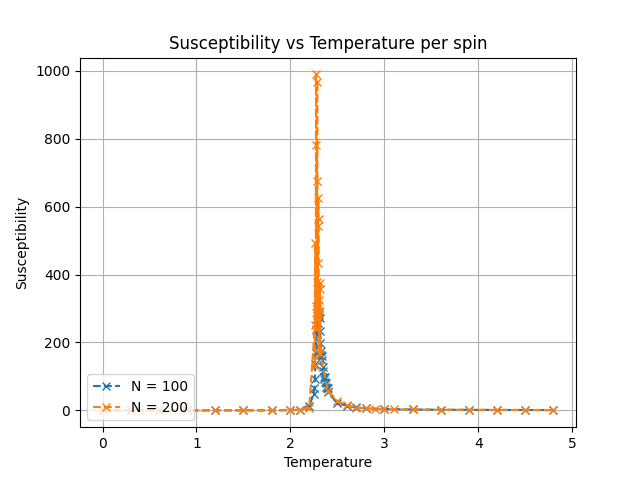
\includegraphics[width=0.75\textwidth]{./resources/susceptibility.png}
\caption{Measured susceptibility versus temperature for two different lattice sizes}
\end{figure}

The peak value is used to calculate the critical temperature and the error is again calculated by the standard deviation between independent simulations. In comparison to the heat capacity, the susceptibility is significantly more peaked and provides a more accurate value for the critical temperature.


\subsection{Finite-Size Scaling}
The argument for finite size scaling of critical temperature relies on the correlation length being limited to the size of the lattice. While the correlation time can grow unbounded, the correlation length which has an assumed power law, \( \xi_{max} \sim (T_c(N) - \kappa)^{-\nu} \sim N \) is bounded by \( N \). This motivates the finite scaling relation
\[ T_c(N) = T_c(\infty) + a N^{-1/\nu} \]

The measured critical temperature versus lattice size is plotted up to \( N = 400 \).

\begin{figure}[H]
\centering
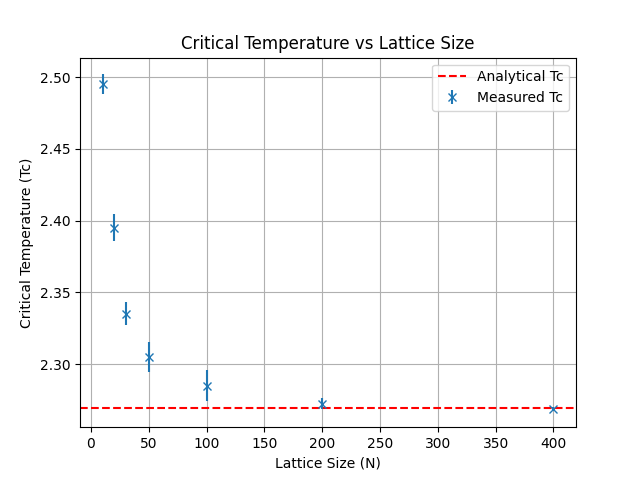
\includegraphics[width=0.75\textwidth]{./resources/finite_size_scaling.png}
\caption{Measured critical temperature versus lattice size}
\end{figure}

In order to estimate the critical temperature for an infinite lattice, the scaling exponent value must be known. According to literature, the 2 dimensional Ising model has \(\nu = 1\) \cite{6}. Therefore the intercept of the plot for critical temperature versus \( 1/N \) will be the desired value.

\begin{figure}[H]
\centering
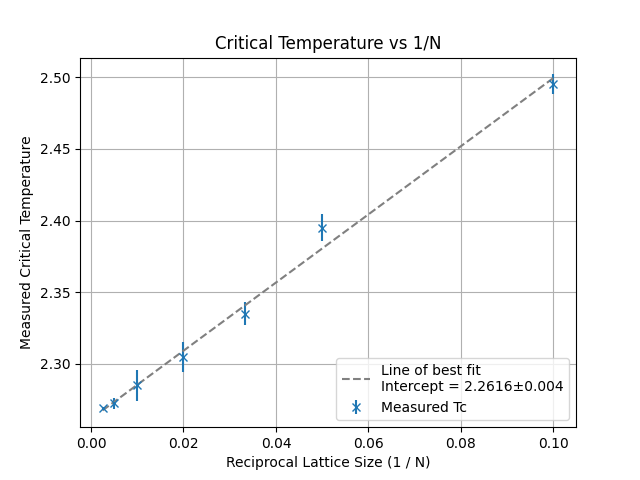
\includegraphics[width=0.75\textwidth]{./resources/infinite_tc_estimate.png}
\caption{Measured critical temperature versus reciprocal lattice size \(1/N\). The line of best fit is shown with the calculated intercept and associated error.}
\end{figure}

From the above plot, the estimated value is \( T_c(\infty) = 2.2616 \pm 0.004\). This result is in agreement with Onsager's analytical value \(T_c \approx 2.269185\) to two decimal places. 

For the largest lattice \(N=400\) the critical temperature was measured as \( T_c ( 400 ) = 2.2690 \pm 0.0015 \). Given the current implementation and hardware, this near the limit of lattice size for which critical temperature can be estimated.


\subsection{Hysteresis}
So far no external field has been present. With the introduction of a variable magnetic field, first order transitions in magnetisation appear as well as hysteresis effects. A magnetic field is added to the simulation and cycled from pointing down to up to down again, with the resulting magnetisation measured. The results for three temperatures are shown below.

\begin{figure}[H]
  \begin{minipage}[t]{0.5\textwidth}
    \captionsetup{width=.8\linewidth}
    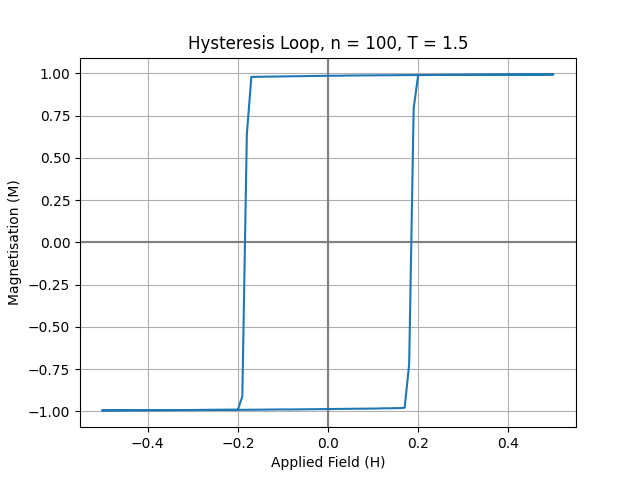
\includegraphics[width=\textwidth]{./resources/hysteresis_T1.5.png}
    \caption{Hysteresis curve for lattice below critical temperature. A first-order discontinuous phase transition in magnetisation occurs, with large coercive field and residual magnetisation.}
  \end{minipage}
  \hfill
  \begin{minipage}[t]{0.5\textwidth}
    \captionsetup{width=.8\linewidth}
    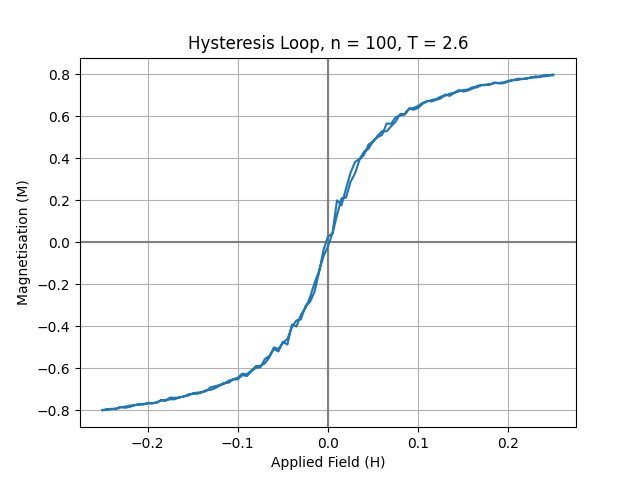
\includegraphics[width=\textwidth]{./resources/hysteresis_T2.6.png}
    \caption{Hysteresis curve for lattice above critical temperature. No phase transition occurs in magnetisation. No hysteresis effect is observed.}
  \end{minipage}
\end{figure}


\begin{figure}[H]
\centering
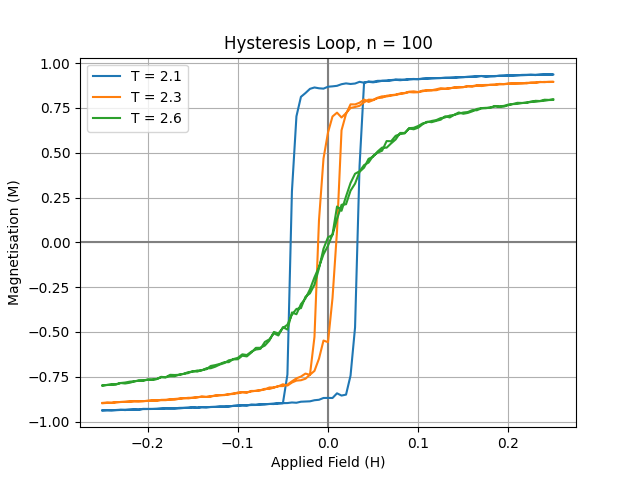
\includegraphics[width=0.75\textwidth]{./resources/loops_overlayed.png}
\caption{Overlayed hysteresis curves for a range of temperatures.}
\end{figure}



\subsection{Spin Visualisation}
The spins of the lattice can be plotted and visualised throughout the simulation. It offers an interesting insight into the processes described above seeing exactly how the crystal reacts.

\newpage
\subsubsection{Cooling}
The process of cooling the lattice through its critical temperature can show qualitatively how the magnetisation breaks symmetry and eventually becomes uniform. Shown below are three frames from the animation file \verb!spins_through_cooling_n500.gif! included in the attached zip file. Black represents spin up, and white spin down, \(N=500\).


\begin{figure}[H]
	\centering
	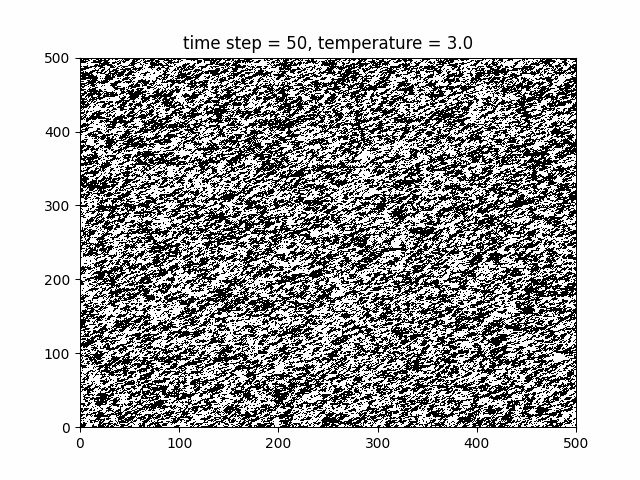
\includegraphics[width=0.5\textwidth]{./resources/frames/cooling_spins_1.jpg}
\end{figure}

\begin{figure}[H]
	\centering
	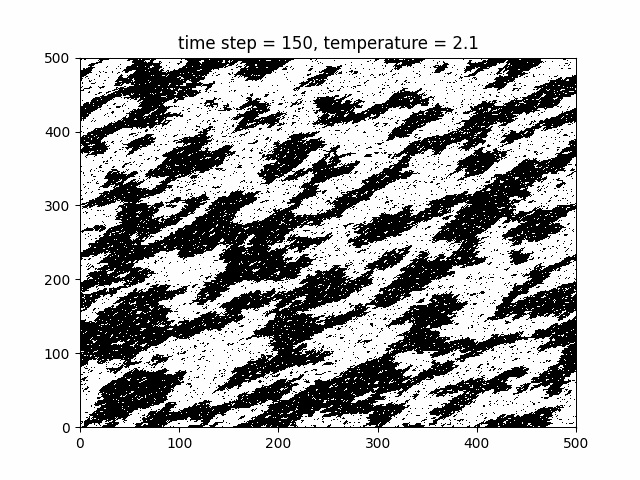
\includegraphics[width=0.5\textwidth]{./resources/frames/cooling_spins_2.jpg}
\end{figure}

\begin{figure}[H]
	\centering
	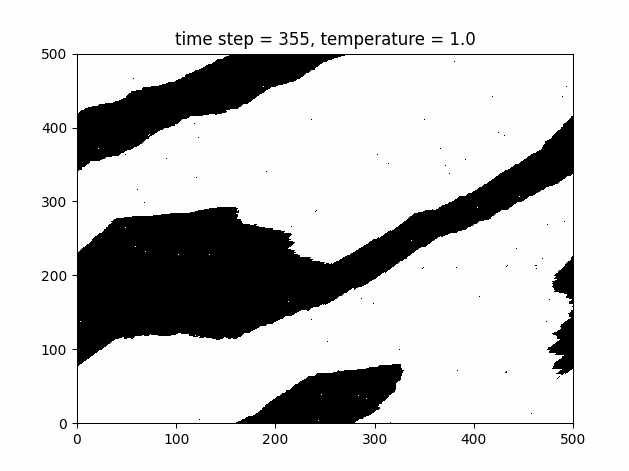
\includegraphics[width=0.5\textwidth]{./resources/frames/cooling_spins_3.png}
\end{figure}


In this simulation, the initial temperature is greater than critical temperature, and the spins appear uniformly distributed with equal spin up and down, magnetisation is zero. In the second frame spin clusters begin to form, however there is still no significant magnetisation apparent. Far below the critical temperature the lattice begins to break symmetry and it is clear the lattice is primarily spin up (white). 

In the final cooling stage, there exists a single spin down cluster (black) which wraps around the edges of the lattice. This is due to the wrap around boundary conditions and corresponds to a single band on the torus. Furthermore, as the second nearest neighbour effects are ignored, the preferred direction for spin clusters to form is diagonally as it minimises energy.

\newpage
\subsubsection{Hysteresis Below Critical Temperature}
The spins of the lattice are now visualised while varying an external magnetic field when the temperature is below the critical point. Shown are frames from the animation file \verb!hysteresis_below_tc_n500.gif! included in the attached zip file.

The left plot displays the spins of the lattice \(N=500\) and the right plot shows the applied magnetic field and the magnetisation.

\begin{figure}[H]
	\centering
	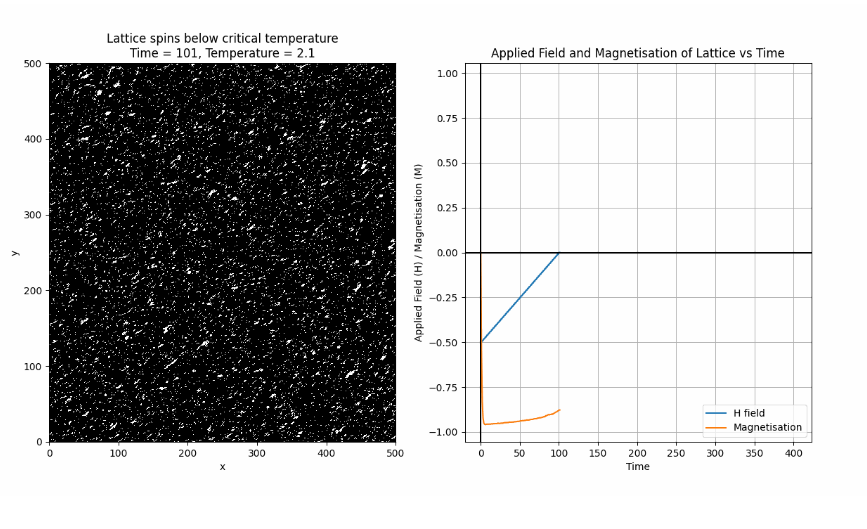
\includegraphics[width=0.8\textwidth]{./resources/frames/hysteresis_below_tc_1.png}
\end{figure}

\begin{figure}[H]
	\centering
	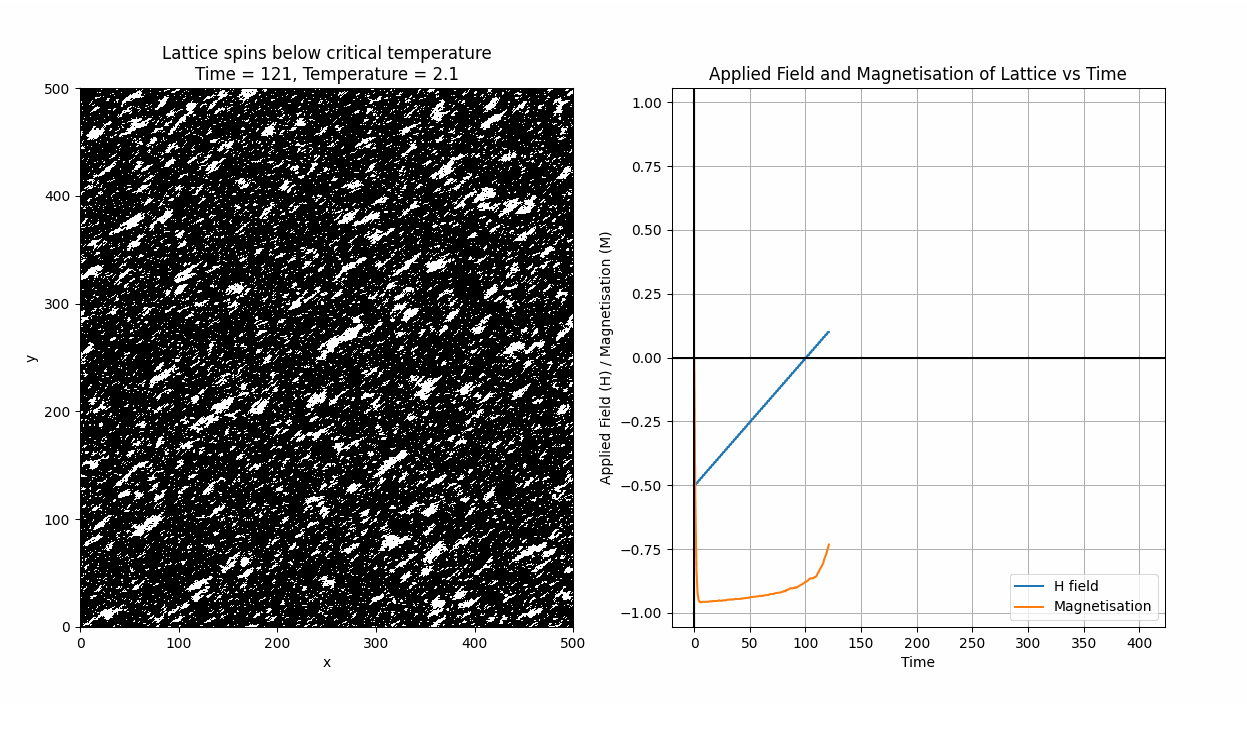
\includegraphics[width=0.8\textwidth]{./resources/frames/hysteresis_below_tc_2.png}
\end{figure}

\begin{figure}[H]
	\centering
	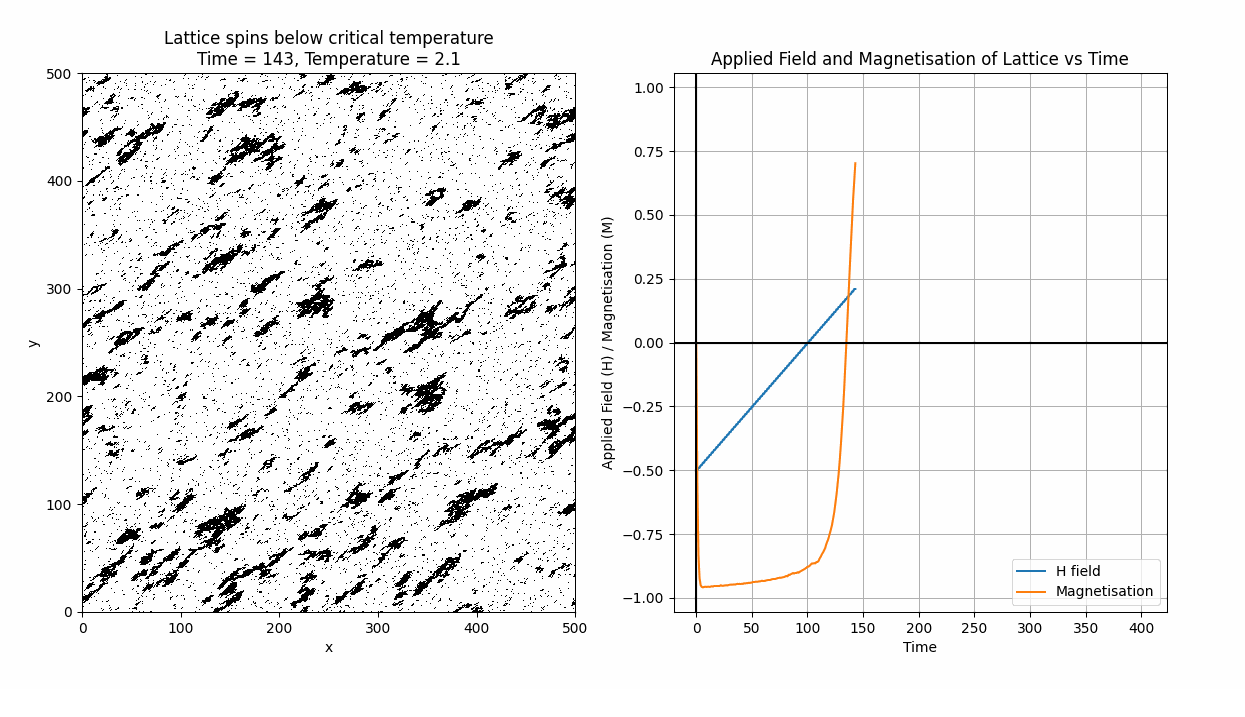
\includegraphics[width=0.8\textwidth]{./resources/frames/hysteresis_below_tc_3.png}
\end{figure}

As the temperature is below the critical value, there is a first order phase transition in magnetisation.

In the first frame the magnetic field has reach zero, and the residual magnetisation can be observed. 

The second frame shows a moment before the phase transition. 

The third frame shows shortly after the phase transition.

\newpage
\subsubsection{Hysteresis Above Critical Temperature}
The same experiment is repeated above the critical temperature. No phase transition in magnetisation is expected. Shown below are three frames from the animation \verb!hysteresis_above_tc_n500.gif! included in the zip attachments.

\begin{figure}[H]
	\centering
	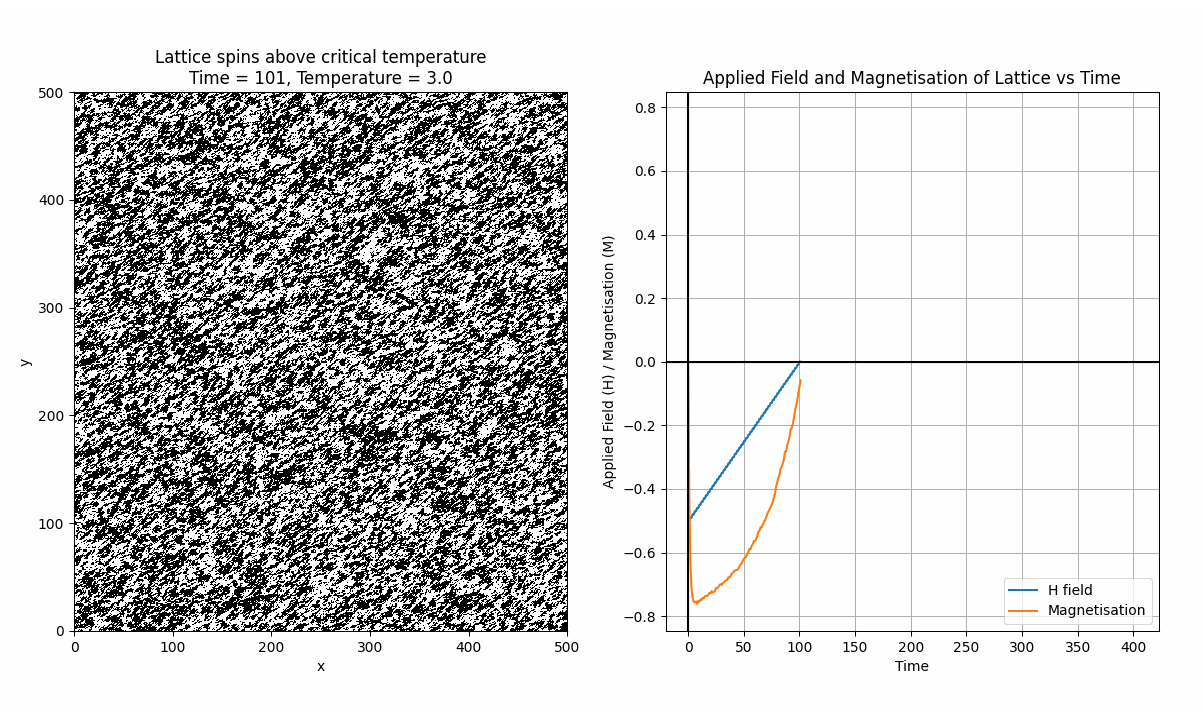
\includegraphics[width=0.8\textwidth]{./resources/frames/hysteresis_above_tc_1.png}
\end{figure}

\begin{figure}[H]
	\centering
	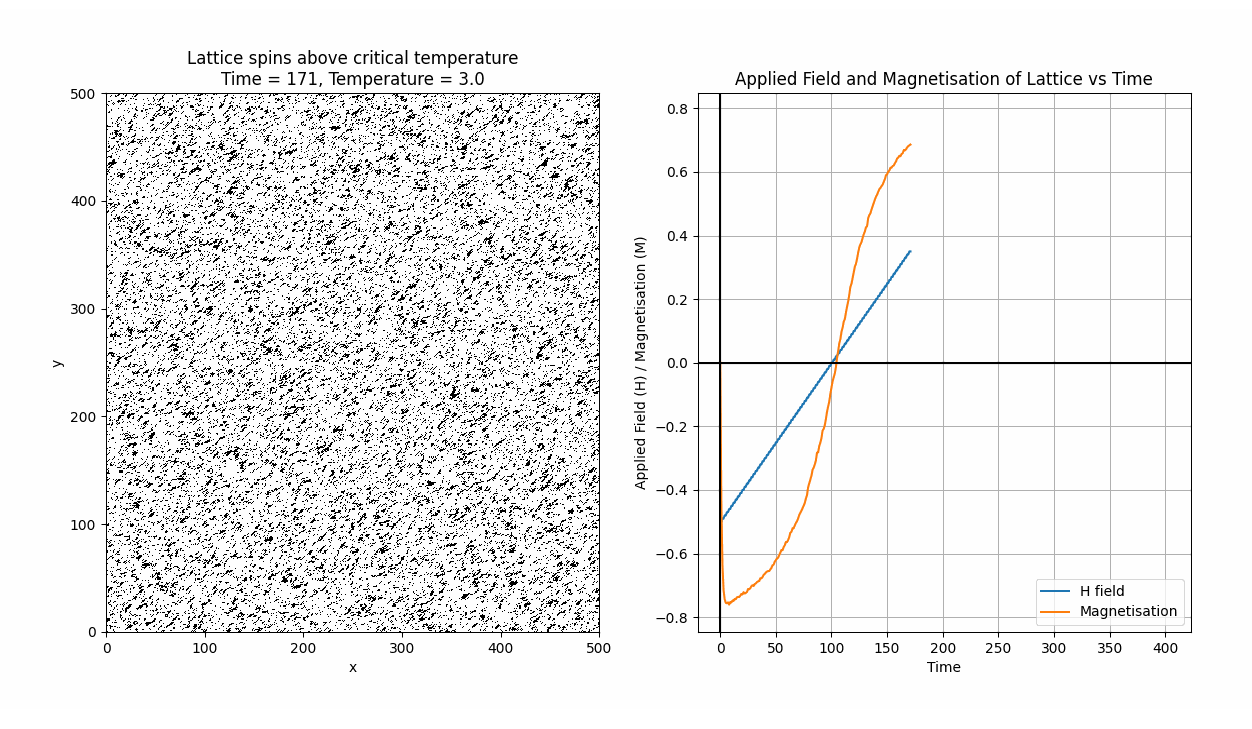
\includegraphics[width=0.8\textwidth]{./resources/frames/hysteresis_above_tc_2.png}
\end{figure}

\begin{figure}[H]
	\centering
	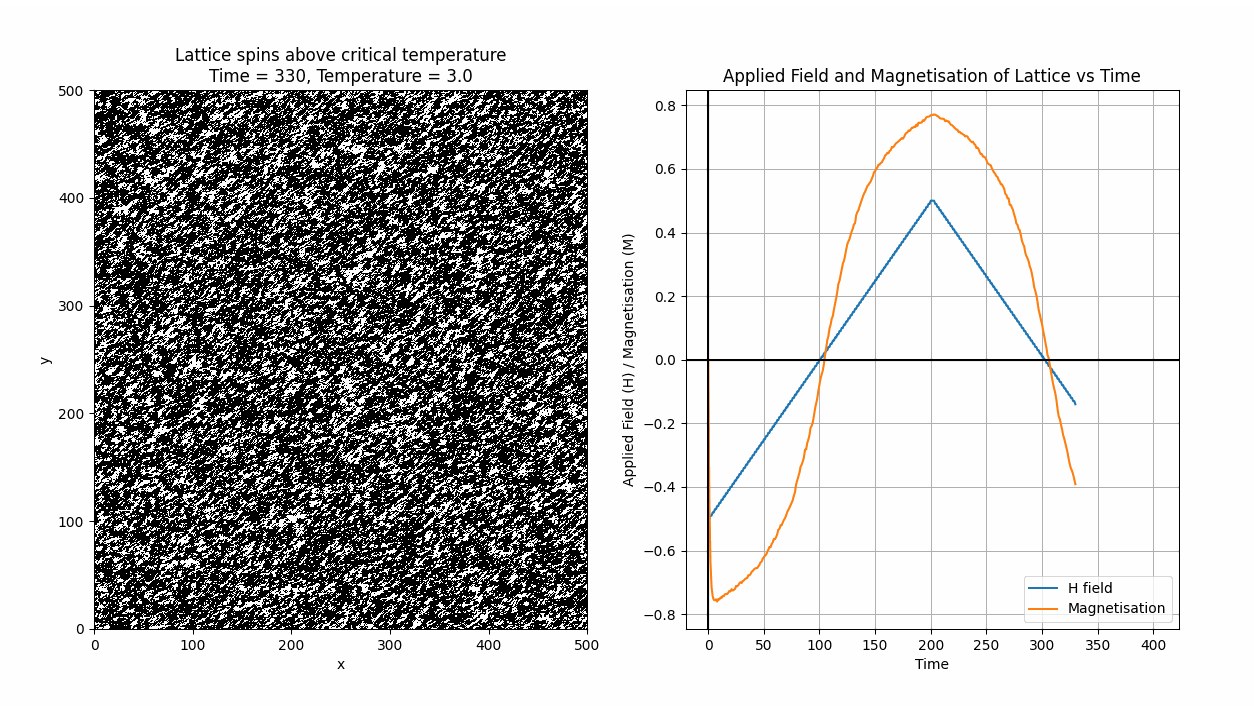
\includegraphics[width=0.8\textwidth]{./resources/frames/hysteresis_above_tc_3.png}
\end{figure}

As predicted, the magnetisation is continuous with magnetic field and time. 

One observation between the two simulations is that at equal magnetisation, the structure of the lattices look very different, comparing above and below critical temperature. Above the critical temperature there are no clusters present and the lattice always looks like "static". In contrast, below the critical temperature there are clusters of spins always present and their scarcity is what impacts the magnetisation.

\section{Conclusion}
The Ising Model provides a very successful statistical model of a ferromagnet. Using the metropolis algorithm and an efficient C++ implementation, many properties of a real ferromagnet were accurately modelled. This includes a continuous second order phase transition in temperature and a first order transition in external field. The results obtained for critical temperature for a lattice size of \(N=400\) was \( T_c = 2.2690 \pm 0.0015 \) which is within Onasger's theoretically obtained value from solving the 2D Ising model analytically. The limitations of the model were also investigated, such as finite size scaling effects and rapidly increasing complexity required for simulating larger lattices. Further work can be done to improve the speed and accuracy of the program, for instance implementing more efficient alternatives to the Metropolis algorithm, such as the Wolff algorithm \cite{7}.

Word count = 2942.

\newpage
\begin{thebibliography}{9}
\bibitem{1}
Onsager, Lars (1944). Crystal statistics. I. A two-dimensional model with an order-disorder transition. https://journals.aps.org/pr/abstract/10.1103/PhysRev.65.117

\bibitem{2}
Fourment, M., \& Gillings, M. R. (2008). A comparison of common programming languages used in bioinformatics. BMC bioinformatics, 9, 82. https://doi.org/10.1186/1471-2105-9-82

\bibitem{3}
M. P. Nightingale (1996). The Dynamic Exponent of the Two-Dimensional Ising Model and Monte Carlo Computation of the Sub-Dominant Eigenvalue of the Stochastic Matrix. https://arxiv.org/abs/cond-mat/9601059

\bibitem{4}
Umberto Marini Bettolo Marconi; Andrea Puglisi; Lamberto Rondoni; Angelo Vulpiani (2008). "Fluctuation-Dissipation: Response Theory in Statistical Physics". https://doi.org/10.1016%2Fj.physrep.2008.02.002

\bibitem{5}
M. Yu. Maslagov (2017). The Analytical Expressions for a Finite-Size 2D Ising Model (2017). The Analytical Expressions for a Finite-Size 2D Ising Model. https://arxiv.org/ftp/arxiv/papers/1706/1706.02541.pdf

\bibitem{6}
N. Crokidakis, I. S. Oliveira (2009). Finite size analysis of a two-dimensional Ising model within a nonextensive approach. https://arxiv.org/abs/0910.2218

\bibitem{7}
Wolff, Ulli (1989). Collective Monte Carlo Updating for Spin Systems. Physical Review Letters. https://doi.org/10.1103%2FPhysRevLett.62.361
\end{thebibliography}


    \newpage

    \appendix
    
    \section{Plotting}
    All plotting was done in Python by reading from data produced by the C++ program. The plotting scripts are included in the zip folder containing attachments. Below is the C++ source code for the numerical routines. In total there is approximately 1000 lines of C++ and 500 lines of Python code. All source code can also be found on GitHub at \href{url}{https://github.com/BorisDeletic/IsingModel}.

    \section{Ising Model Source Code}
\subsection{lattice.h}
\begin{lstlisting}
//
// Created by boris on 07/03/2022.
//

#ifndef ISINGMODEL_LATTICE_H
#define ISINGMODEL_LATTICE_H

#include <vector>
#include <iostream>

using namespace std;

class Lattice {
public:
    Lattice(int n);

    void randomize();
    double magnetisation();
    double energy(float H);

    vector<vector<signed char>> spins;

    friend ostream& operator << (ostream &o, const Lattice &l);

private:
    int n;
};

#endif //ISINGMODEL_LATTICE_H
\end{lstlisting}
    
 \newpage
\subsection{lattice.cpp}
\begin{lstlisting}
    #include "lattice.h"
#include <stdlib.h>


Lattice::Lattice(int n)
    :
    n(n),
    spins(vector<vector<signed char>>(n, vector<signed char>(n, 1)))
{

}


void Lattice::randomize() {
    for (int i = 0; i < n; i++)
    {
        for (int j = 0; j < n; j++)
        {
            signed char spin = rand() % 2 == 0 ? 1 : -1;
            spins[i][j] = spin;
        }
    }
}



double Lattice::magnetisation() {
    double mag = 0;

    for (int i = 0; i < n; i++)
    {
        for (int j = 0; j < n; j++)
        {
            mag += spins[i][j];
        }
    }
    return mag;
}


double Lattice::energy(float H) {
    double energy = 0;

    for (int i = 0; i < n; i++) {
        for (int j = 0; j < n; j++) {
            signed char s0 = spins[i][j];

            // get neighbour spins and use wrap-around boundary conditions
            signed char s1 = spins[i - 1 >= 0 ? i - 1 : n - 1][j];
            signed char s2 = spins[i + 1 < n ? i + 1 : 0][j];
            signed char s3 = spins[i][j - 1 >= 0 ? j - 1 : n - 1];
            signed char s4 = spins[i][j + 1 < n ? j + 1 : 0];

            double neighbours = (s0 * s1) + (s0 * s2) + (s0 * s3) + (s0 * s4);
            double Hterm = H * s0;

            energy += -neighbours - Hterm;
        }
    }

    return energy;
}



ostream &operator<<(ostream &o, const Lattice &l) {
    for (int i = 0; i < l.spins.size(); i++) {
        for (int j = 0; j < l.spins.size(); j++) {
            o << (int)l.spins[i][j] << "\t";
        }
        o << endl;
    }

    return o;
}
\end{lstlisting}


\newpage
\subsection{engine.h}
\begin{lstlisting}
//
// Created by boris on 10/03/2022.
//

#ifndef ISINGMODEL_ENGINE_H
#define ISINGMODEL_ENGINE_H

#include <random>
#include "lattice.h"

class Engine {
public:
    Engine(int n);

    void timeStep(Lattice& lattice);
    double fluctuations(vector<double>& quantity, int t0);

    void setTemperature(float temperature) {T = temperature; };
    void setHField(float field) {H = field; };
    float getTemperature() { return T; };
    float getHField() { return H; };

    bool monteCarlo = false;
private:
    void calculateNewSpinsMC(vector<vector<signed char>>& newSpins);
    void calculateNewSpinsLA(vector<vector<signed char>>& newSpins);
    signed char flipSpin(signed char s0, vector<signed char> neighbours);

    int n;
    float T;
    float H;

    random_device rd;  // Will be used to obtain a seed for the random number engine
    mt19937 gen; // Standard mersenne_twister_engine seeded with rd()
    uniform_real_distribution<> tempRNG; //random numbers for temperature effect
    uniform_int_distribution<> spinRNG; //rng for selecting lattice site
};


#endif //ISINGMODEL_ENGINE_H
\end{lstlisting}

\newpage
\subsection{engine.cpp}
\begin{lstlisting}
#pragma clang diagnostic push
#pragma ide diagnostic ignored "openmp-use-default-none"
//
// Created by boris on 10/03/2022.
//

#include <math.h>
#include <algorithm>
#include "engine.h"
#include "lattice.h"


Engine::Engine(int n)
    :
    n(n),
    T(0),
    H(0),
    gen(rd()),
    tempRNG(0.0, 1.0), //setup random number generator
    spinRNG(0, n-1)
{
}


void Engine::timeStep(Lattice& lattice)
{
    if (monteCarlo) {
        calculateNewSpinsMC(lattice.spins);
    } else {
        calculateNewSpinsLA(lattice.spins);
    }
}


//calculate linearly going through lattice
void Engine::calculateNewSpinsLA(vector<vector<signed char>> &newSpins)
{
    for (int i = 0; i < n; i++) {
        for (int j = 0; j < n; j++) {
            signed char s0 = newSpins[i][j];

            // get neighbour spins and use wrap-around boundary conditions
            signed char s1 = newSpins[i - 1 >= 0 ? i - 1 : n - 1][j];
            signed char s2 = newSpins[i + 1 < n ? i + 1 : 0][j];
            signed char s3 = newSpins[i][j - 1 >= 0 ? j - 1 : n - 1];
            signed char s4 = newSpins[i][j + 1 < n ? j + 1 : 0];

            newSpins[i][j] = flipSpin(s0, {s1, s2, s3, s4});
        }
    }
}

// pick spins to flip randomly
void Engine::calculateNewSpinsMC(vector<vector<signed char>> &newSpins)
{

    for (int t = 0; t < n * n; t++) {
        int i = spinRNG(gen);
        int j = spinRNG(gen);

        signed char s0 = newSpins[i][j];

        // get neighbour spins and use wrap-around boundary conditions
        signed char s1 = newSpins[i - 1 >= 0 ? i - 1 : n - 1][j];
        signed char s2 = newSpins[i + 1 < n ? i + 1 : 0][j];
        signed char s3 = newSpins[i][j - 1 >= 0 ? j - 1 : n - 1];
        signed char s4 = newSpins[i][j + 1 < n ? j + 1 : 0];

        newSpins[i][j] = flipSpin(s0, {s1, s2, s3, s4});
    }
}


signed char Engine::flipSpin(signed char s0, vector<signed char> neighbours) {
    int sFlipped = s0 == 1 ? -1 : 1;

    float neighbourTerm = 0.0f;
    float neighbourTermFlipped = 0.0f;
    for (int i = 0; i < 4; i++)
    {
        neighbourTerm += s0 * neighbours[i];
        neighbourTermFlipped += sFlipped * neighbours[i];
    }

    float Enow = - neighbourTerm - H * s0;
    float Eflip = - neighbourTermFlipped - H * sFlipped;

    float deltaE = Eflip - Enow;

    if (deltaE < 0.0f) { // flip the spin
        return sFlipped;
    }

    double thermalEnergy = exp(- deltaE / T);
    double threshold = tempRNG(gen);

    if (thermalEnergy > threshold)
    {
        return sFlipped;
    }

    return s0;
}


double Engine::fluctuations(vector<double>& quantity_raw, int t0)
{
    vector<double> quantity;
    for (double q : quantity_raw) {
        quantity.push_back(fabs(q));
    }

    const int len = quantity.size() - t0;

    double mean = reduce(quantity.begin() + t0, quantity.end()) / len;

    vector<double> rmsQuantity;

    for (int i = t0; i < quantity.size(); i++) {
        double rms = pow(quantity[i] - mean, 2);
        rmsQuantity.push_back(rms);
    }

    double variance = reduce(rmsQuantity.begin(), rmsQuantity.end()) / rmsQuantity.size();

    return variance;
}


#pragma clang diagnostic pop
\end{lstlisting}



\newpage
\subsection{simulation.h}
\begin{lstlisting}
//
// Created by boris on 10/03/2022.
//

#ifndef ISINGMODEL_SIMULATION_H
#define ISINGMODEL_SIMULATION_H

#include <optional>
#include "engine.h"
#include "lattice.h"

class Simulation {
public:
    Simulation(int n);

    void run(int timeSteps);

    optional<int> timeToEquilibrium();

    void setTemperature(float T) { engine.setTemperature(T); };
    void setHField(float H) { engine.setHField(H); };
    float getTemperature() { return engine.getTemperature(); };
    float getHField() { return engine.getHField(); };

    void randomize(void) { randomised = true; lattice.randomize(); };

    friend ostream& operator << (ostream &o, const Simulation &l);

    // properties
    Engine engine;
    Lattice lattice;

    vector<double> magnetisations;
    vector<double> energy;
    vector<double> flips;

    int n;
    bool randomised = false;
    const float correlationCutoff = 0.2;

};


#endif //ISINGMODEL_SIMULATION_H
\end{lstlisting}

\newpage
\subsection{simulation.cpp}
\begin{lstlisting}
//
// Created by boris on 10/03/2022.
//

#include <iostream>
#include <algorithm>
#include "simulation.h"

using namespace std;

double gradientLineBestFit(const std::vector<double> &pts);

Simulation::Simulation(int n)
    :
    engine(n),
    lattice(n),
    n(n),
    magnetisations(),
    flips()
{
}


void Simulation::run(int timeSteps)
{
    for (int i = 0; i < timeSteps; i++) {
        magnetisations.push_back(lattice.magnetisation());
        energy.push_back(lattice.energy(getHField()));

        engine.timeStep(lattice);
    }
}


optional<int> Simulation::timeToEquilibrium() {
/*
 * Calculate the number of steps before energy stabilises -> equilibrium
 * We consider energy stabilised when the line of best fit is flat.
 * Only looking at the energy in a window (1/10th of the total time).
 */
    const int steps = energy.size();

    const int windowSize = steps / 10;
    const float slopeThreshold = 0.0005;

     for (int i = windowSize; i < steps - windowSize; i+=5) {
         auto start = energy.begin() + i;
         auto end = energy.begin() + i + windowSize;

        vector<double> window;
        for (auto it = start; it < end; it++)
        {
            window.push_back(*it / (n*n)); //fractional magnetisation
        }

        double slope = gradientLineBestFit(window);

        if (abs(slope) < slopeThreshold) {
            return i;
        }
    }

    // equilibrium conditions not reached
    return nullopt;
}


double gradientLineBestFit(const vector<double> &pts)
{
    int nPoints = pts.size();
    if( nPoints < 2 ) {
        return 0;
    }
    double sumX=0, sumY=0, sumXY=0, sumX2=0;
    for(int i=0; i<nPoints; i++) {
        sumX += i;
        sumY += pts[i];
        sumXY += i * pts[i];
        sumX2 += i * i;
    }
    double xMean = sumX / nPoints;
    double yMean = sumY / nPoints;
    double denominator = sumX2 - sumX * xMean;
    // You can tune the eps (1e-7) below for your specific task
    if( fabs(denominator) < 1e-7 ) {
        // Fail: it seems a vertical line
        return 1e7;
    }
    double slope = (sumXY - sumX * yMean) / denominator;

    return slope;
}




ostream &operator<<(ostream &o, const Simulation &s) {
    o << "Simulation Parameters:" << endl;
    o << "n = " << s.n << endl;
    o << "steps = " << s.magnetisations.size() << endl;

    return o;
}

\end{lstlisting}


\newpage
\section{Simulations Source Code}
\subsection{analysis.h}
\begin{lstlisting}
//
// Created by boris on 29/03/2022.
//

#ifndef ISINGMODEL_ANALYSIS_H
#define ISINGMODEL_ANALYSIS_H

#include <vector>
#include <optional>
#include "../src/simulation.h"

using namespace std;

struct Results
{
    int n;
    float T;
    float H = 0.0;
    bool randomised;

    int equilibriumTime;
    int decorrelationTime;

    double meanMagnetisation;
    double spinVariance;

    double heatCapacity;
    double energyVariance;

    vector<double> magnetisations;
    vector<double> energys;
    vector<double> correlations;
};


class Analysis {
public:
    Analysis();

    void calculateResults(Simulation& sim);


    // DECORRELATIONS //
    static optional<int> decorrelationTime(vector<double>& autoCorrelation);
    static vector<double> autoCorrelations(vector<double>& mags, int t0);
    static double autoCovariance(vector<double>& mags, int t_start, int tau);


    void logResults();

    string fname = R"(..\results\zero_field.csv)";
private:
    Results results;
};


#endif //ISINGMODEL_ANALYSIS_H
\end{lstlisting}


\newpage
\subsection{analysis.cpp}
\begin{lstlisting}
//
// Created by boris on 29/03/2022.
//

#include <algorithm>
#include <fstream>
#include "analysis.h"



Analysis::Analysis()
{
    ifstream f(fname);
    if (!f.good())
    {
        ofstream file;
        file.open(fname);

        file << "n, T, randomised, equilibriumTime, decorrelationTime, meanMagnetisation, spinVariance, heatCapacity, energyVariance" << endl;
        file << "magnetisations" << endl;
        file << "energys" << endl;
        file << "correlations" << endl;

        file.close();
    }
}


void Analysis::calculateResults(Simulation &sim) {
    float T = sim.getTemperature();

    optional<int> t_eq = sim.timeToEquilibrium();
    if (!t_eq) {
        // equilibrium conditions not reached
        printf("Equilibrium not reached in %d steps from absMags\n", sim.magnetisations.size());
        throw std::exception();
    }

    vector<double> correlations = autoCorrelations(sim.magnetisations, *t_eq);
    optional<int> decorTime = decorrelationTime(correlations);

    if (!decorTime) {
        printf("Did not decorrelate in %d steps\n", sim.magnetisations.size());
        throw std::exception();
    }

    int len = sim.magnetisations.size();

    // find mean of |M| instead of M
    double meanMag = 0;
    vector<double> absMags;
    for (int i = *t_eq; i < len; i++) {
        meanMag += fabs(sim.magnetisations[i]);
    }
    meanMag /= len - *t_eq;

    results.n = sim.n;
    results.T = T;
    results.H = sim.getHField();
    results.randomised = sim.randomised ? 1 : 0;

    results.equilibriumTime = *t_eq;
    results.decorrelationTime = *decorTime;

    results.meanMagnetisation = meanMag;
    results.spinVariance = sim.engine.fluctuations(sim.magnetisations, *t_eq);

    results.energyVariance = sim.engine.fluctuations(sim.energy, *t_eq);
    results.heatCapacity = T == 0 ? 0 : results.energyVariance / (pow(T, 2));

    results.magnetisations = sim.magnetisations;
    results.energys = sim.energy;
    results.correlations = correlations;
}



// DECORRELATIONS //
vector<double> Analysis::autoCorrelations(vector<double>& mags, int t0)
{
    float correlationCutoff = 0.2;
    // the maximum offset we can calculate correlation for is 20% of total time

    double autoCov0 = autoCovariance(mags, t0, 0);
    vector<double> autoCors;

    float maxTau = (mags.size() - t0) * correlationCutoff;

    for (int tau = 0; tau < maxTau; tau++)
    {
        double cor = autoCovariance(mags, t0, tau) / autoCov0;

        cor = autoCov0 == 0 ? 0 : cor;
        autoCors.push_back(cor);
    }

    return autoCors;
}


double Analysis::autoCovariance(vector<double>& mags, int t_start, int tau)
{
    double meanMagnetisation = reduce(mags.begin() + t_start, mags.end()) / (mags.size() - t_start);

    vector<double> covariance;

    for (int i = t_start; i < mags.size() - tau; i++)
    {
        double magP = mags[i] - meanMagnetisation;
        double magP_tau = mags[i + tau] - meanMagnetisation;

        covariance.push_back(magP * magP_tau);
    }

    double meanCov = reduce(covariance.begin(), covariance.end()) / covariance.size();

    return meanCov;
}


//   Decorrelation time is how long before auto correlation falls to 1/e
optional<int> Analysis::decorrelationTime(vector<double>& autoCorrelation)
{
    double decayValue = 0.367879441;

    for (int i = 0; i < autoCorrelation.size(); i++)
    {
        if (autoCorrelation[i] < decayValue) {
            return i;
        }
    }

    return nullopt;
}

//////////////////////////////////////////////////////////////////////////////


void Analysis::logResults()
{
    int rand = results.randomised ? 1 : 0;

    ofstream file;
    file.open(fname, fstream::app);

    file <<
        results.n << "," <<
        results.T << "," <<
        results.H << "," <<
        rand << "," <<
        results.equilibriumTime << "," <<
        results.decorrelationTime << "," <<
        results.meanMagnetisation << "," <<
        results.spinVariance << "," <<
        results.heatCapacity << "," <<
        results.energyVariance << "," << endl;


    for (double mag : results.magnetisations)
    {
        file << mag << ",";
    }
    file << endl;

    for (double energy : results.energys)
    {
        file << energy << ",";
    }
    file << endl;

    for (double correlation : results.correlations)
    {
        file << correlation << ",";
    }
    file << endl;

    file.close();
}
\end{lstlisting}


\newpage
\subsection{hysteresis.h}
\begin{lstlisting}
//
// Created by Boris Deletic on 28/03/2022.
//

#ifndef ISINGMODEL_HYSTERESIS_H
#define ISINGMODEL_HYSTERESIS_H

#include <vector>

void runHysteresisLoop(int n, float T, std::vector<float>& Hs);

#endif //ISINGMODEL_HYSTERESIS_H

\end{lstlisting}



\newpage
\subsection{hysteresis.cpp}
\begin{lstlisting}
//
// Created by Boris Deletic on 28/03/2022.
//

#include <fstream>
#include "hysteresis.h"
#include "../src/simulation.h"



void runHysteresisLoop(int n, float T, vector<float>& Hs)
{
    ofstream file;
    file.open(R"(..\results\hysteresis.csv)", fstream::app);

    file << n << "," << T << endl;

    int initSteps = 500;
    int steps = 100;


    Simulation sim(n);
    sim.setTemperature(T);
    sim.setHField(Hs[0]);

    sim.run(initSteps);

    for (int i = 0; i < Hs.size(); i++)
    {
        float H = Hs[i];
        sim.setHField(H);
        sim.run(steps);

        int start = sim.magnetisations.size() - steps;

        vector<double> mags;
        for (int i = start; i < sim.magnetisations.size(); i++) {
            mags.push_back(sim.magnetisations[i]);
        }

        double meanMag = reduce(mags.begin(), mags.end()) / mags.size();

        file << H << "," << meanMag << endl;

        cout << sim;
        cout << "T = " << sim.getTemperature() << endl;
        cout << "H = " << sim.getHField() << endl << endl;

    }

    file << endl;
    file.close();

}
\end{lstlisting}



\newpage
\subsection{run.h}
\begin{lstlisting}
//
// Created by boris on 23/03/2022.
//

#ifndef ISINGMODEL_RUN_H
#define ISINGMODEL_RUN_H


#include "../src/simulation.h"

void runZeroFieldSimulations();
void runFieldSimulations(float H);
void runSpinsWithCooling();
void runSpinsWithHField(float T);

void runSim(Simulation& sim, float T, int steps, bool randomised);

const int maxSteps = 200000;
const int initSteps = 5000;


#endif //ISINGMODEL_RUN_H

\end{lstlisting}


\newpage
\subsection{run.cpp}
\begin{lstlisting}
//
// Created by boris on 23/03/2022.
//

#include <set>
#include "run.h"
#include "spins_logger.h"
#include "analysis.h"

void runZeroFieldSimulations()
{
   const int reps = 10;
   set<int> Ns = {10, 20, 30, 50, 100, 200};
   set<float> Ts;

    for (float T = 0; T < 5; T+=0.3) {
        Ts.insert(T);
    }
    for (float T = 2.25; T < 3.3; T+=0.05) {
        Ts.insert(T);
    }

// for large n
  //  Ts.insert(2.2692);
  //  Ts.insert(2.2695);
   // Ts.insert(2.271);
  //  Ts.insert(2.269);
//    for (float T = 2.269; T < 2.274; T += 0.001) {
//        Ts.insert(T);
//    }
//    for (float T = 2.0; T < 3.101; T += 0.1) {
//        Ts.insert(T);
//    }

    for (int i = 0; i < reps; i++) {
        for (int n: Ns) {
            for (float T: Ts) {
                Simulation sim(n);
                Analysis nofield;

                runSim(sim, T, initSteps, false);

                nofield.calculateResults(sim);
                nofield.logResults();
            }
        }
    }
}


void runFieldSimulations(float H)
{
    const int reps = 5;
    int n = 100;
    set<float> Ts;

    for (float T = 0; T < 10; T+=0.3) {
        Ts.insert(T);
    }

    for (int i = 0; i < reps; i++) {
        for (float T: Ts) {
            Simulation sim(n);
            sim.setHField(H);

            Analysis nonzerofield;
            nonzerofield.fname = R"(..\results\H_field.csv)";

            runSim(sim, T, initSteps, false);

            nonzerofield.calculateResults(sim);
            nonzerofield.logResults();
        }
    }
}





void runSim(Simulation& sim, float T, int steps, bool randomised)
{
    if (randomised) sim.randomize();
    sim.setTemperature(T);

    int decorTimeFactor = 10;
    int minSteps = maxSteps;
    optional<int> t_eq;
    optional<int> decorTime;

    //while steps < minSteps
    while (sim.magnetisations.size() < minSteps || !t_eq || !decorTime)
    {
        sim.run(steps);
        t_eq = sim.timeToEquilibrium();

        if (t_eq) {

            vector<double> correlations = Analysis::autoCorrelations(sim.magnetisations, *t_eq);
            decorTime = Analysis::decorrelationTime(correlations);

            if (decorTime) {
                minSteps = *decorTime * decorTimeFactor;
                minSteps = minSteps < maxSteps ? minSteps : maxSteps; // cap min steps at the maximum allowed
            }
        }

        steps *= 1.5;

        if (sim.magnetisations.size() > maxSteps) {
            printf("Equilibrium not reached in %d steps from main\n", sim.magnetisations.size());
            throw std::exception();
        }
    }


    cout << sim;
    cout << "T = " << T << endl;
    cout << "H = " << sim.getHField() << endl;
    cout << "steps to decorrelate = " << *decorTime << endl;
    cout << "steps to eq = " << *t_eq << endl << endl;
}



void runSpinsWithCooling()
{
    int n = 100;
    int steps = 100;
    vector<float> Ts = {3, 2.1, 1.0};

    SpinLogger logger(n, steps * Ts.size());

    Simulation sim(n);
    cout << sim;


    for (float T : Ts) {
        sim.setTemperature(T);
        for (int i = 0; i < steps; i++) {
            sim.run(1);

            logger.logSpins(sim);
        }
    }
}


void runSpinsWithHField(float T)
{
    int n = 500;
    int steps = 2;
    vector<float> Hs;
    for (float H = -0.5; H < 0.5; H+=0.01) {
        Hs.push_back(H);
    }
    for (float H = 0.5; H > -0.5; H-=0.01) {
        Hs.push_back(H);
    }

    SpinLogger logger(n, steps * Hs.size());

    Simulation sim(n);
    sim.randomize();
    sim.setTemperature(T);
    cout << sim;

    for (float H : Hs) {
        sim.setHField(H);
        for (int i = 0; i < steps; i++) {
            sim.run(1);

            logger.logSpins(sim);
        }

        cout << sim;
    }
}
\end{lstlisting}

\newpage
\subsection{spins\_logger.h}
\begin{lstlisting}
//
// Created by boris on 27/03/2022.
//

#ifndef ISINGMODEL_SPINS_H
#define ISINGMODEL_SPINS_H

#include <vector>
#include "../src/simulation.h"

class SpinLogger {
public:
    void logSpins(Simulation& sim);

    SpinLogger(int n, int steps);

private:
    string fname = R"(..\results\spins.csv)";
};


#endif //ISINGMODEL_SPINS_H
\end{lstlisting}


\newpage
\subsection{spins\_logger.cpp}
\begin{lstlisting}
//
// Created by boris on 27/03/2022.
//

#include "spins_logger.h"
#include <fstream>


SpinLogger::SpinLogger(int n, int steps)
{
    ofstream myfile;
    myfile.open(fname);

    myfile << n << "," << steps << endl;
    myfile.close();
}


void SpinLogger::logSpins(Simulation &sim) {
    int n = sim.lattice.spins.size();
    float T = sim.getTemperature();
    float H = sim.getHField();
    double mag = sim.magnetisations[sim.magnetisations.size() - 1];

    ofstream myfile;
    myfile.open(fname, fstream::app);

    myfile << T << "," << H << "," << mag << endl;

    for (int i = 0; i < n; i++) {
        for (int j = 0; j < n; j++) {
            myfile << (int)sim.lattice.spins[i][j] << ",";
        }
    }
    myfile << endl;

    myfile.close();
}

\end{lstlisting}



\newpage
\subsection{main.cpp}
\begin{lstlisting}

#include <fstream>
#include <chrono>
#include "simulations/hysteresis.h"
#include "simulations/run.h"

using namespace std;


void measureSpeed();
void hysteresis();

int main()
{

    runZeroFieldSimulations();

    //runSpinsWithCooling();
 //   runSpinsWithHField(2.1);

//    vector<float> Hs = {0.1, 0.2, 0.4, 0.6, 0.8, 1.0, 1.5, 2.0};
//    for (float H : Hs) {
//        runFieldSimulations(H);
//    }
 //   measureSpeed();
}


void hysteresis()
{
    vector<float> Hs;
    vector<float> Hs2;
    for (float H = -0.25; H <= 0.25; H+=0.005) {
        Hs.push_back(H);
    }

    for (float H = -0.5; H <= 0.5; H+=0.01) {
        Hs2.push_back(H);
    }

    runHysteresisLoop(100, 2.1, Hs);
    runHysteresisLoop(100, 2.2, Hs);
    runHysteresisLoop(100, 2.3, Hs);
    runHysteresisLoop(100, 2.6, Hs);
    runHysteresisLoop(100, 1.5, Hs2);

}

void measureSpeed()
{
    ofstream file;
    file.open(R"(..\results\speed.csv)");

    // should take approx 12h
    vector<int> Ns = {10, 20, 50, 100, 200, 300, 400, 500, 600, 700, 800, 900, 1000};
    int steps = 10000;


    for (int montecarlo = 0; montecarlo < 2; montecarlo++) {
        for (int n : Ns) {
            auto t1 = std::chrono::high_resolution_clock::now();

            Simulation sim(n);
            sim.engine.monteCarlo = !(montecarlo == 0);
            sim.run(steps);

            auto t2 = std::chrono::high_resolution_clock::now();

            /* Getting number of milliseconds as an integer. */
            auto time = std::chrono::duration_cast<std::chrono::milliseconds>(t2 - t1);

            file << n << "," << montecarlo << "," << steps << "," << time.count() << endl;

            cout << sim << endl;
        }
    }

    file.close();
}
\end{lstlisting}

\end{document}
